\documentclass[10pt]{book}

\usepackage{amsmath}
\usepackage{amssymb}
\usepackage{amsfonts}
\usepackage[mathscr]{euscript}
\usepackage{wasysym}	% cent symbol \cent
\usepackage[T1]{fontenc}
\usepackage{etoolbox}
\usepackage{qrcode}

\newtoggle{solutions}
\toggletrue{solutions}
\togglefalse{solutions}


%	%	%	%	%	%
%	Look & Layout	%
%	%	%	%	%	%

\usepackage[margin=1in]{geometry}

\usepackage{titlesec}
\titleformat{\chapter}[hang]{\LARGE\bfseries}{%
  \thechapter\hspace{1em}}{0pt}{\LARGE\bfseries} % Compact Chapter title
\titlespacing{\chapter}{0pt}{0pt}{0pt}	% Eliminate space before/after
% chapter
%\pagestyle{empty}
\usepackage{fancyhdr}
\pagestyle{fancy}
\lfoot{Page \thepage}
\rfoot{~}
\cfoot{~}


\linespread{1.1}
\everymath{\displaystyle}
\setlength{\parindent}{0pt}

\usepackage{multicol}
\setlength{\columnsep}{30pt}
%\setlength\columnseprule{0.4pt}
\raggedcolumns

\usepackage[inline,shortlabels]{enumitem} % For inline lists
\usepackage{etoolbox}

\usepackage{tikz}
\usetikzlibrary{calc}	% For calculating coordinates e.g. ($ (P)+(\xlength,\height) $)
\usetikzlibrary{positioning}
\usetikzlibrary{decorations.markings}
\usetikzlibrary{matrix}

\usepackage{pgfplots}
% As of 1.11, you may write tikz coordinates as (2,1) rather than having to type (axis cs:2,1)
\pgfplotsset{compat=1.11}

\newcommand{\Rand}{\pgfmathparse{random(7)}\pgfmathresult}

\newcommand{\boxcolor}{gray!30}
\usepackage{mdframed}
\newenvironment{boxme}{\begin{mdframed}[backgroundcolor=\boxcolor,linewidth=0pt,nobreak=true]}{\end{mdframed}}
\newenvironment{boxthm}{\begin{mdframed}[backgroundcolor=\boxcolor,nobreak=true]}{\end{mdframed}}
\newenvironment{boxdef}{\begin{mdframed}[backgroundcolor=\boxcolor,linewidth=0pt,nobreak=true]}{\end{mdframed}}


%	%	%	%	%	%	%	%
%	Exercise Environment	%
%	%	%	%	%	%	%	%

\usepackage{amsthm}

\newtheorem*{theorem}{Theorem}

\theoremstyle{definition}
\newtheorem{exercise}{Exercise}[section]
\newtheorem{problem}{Problem}[section]
\renewcommand{\theexercise}{\arabic{exercise}}	% Shows Exercise 2
\renewcommand{\theproblem}{\arabic{problem}}	% Shows Problem 2 instead of Problem 1.1.2


%	%	%	%	%	%	%	%	%	%	%
%	Systems of Equations and Matrices	%
%	%	%	%	%	%	%	%	%	%	%

\usepackage{systeme}
%\syslineskipcoeff{1.2}\setlength{\tabskip}{3pt}
%\systeme{
%	2x  +   y  +  3z  =  10,
%	x  +   y  +   z  =   6,
%	x  +  3y  +  2z  =  13}

% Right align RHS of systeme
\makeatletter
\def\SYS@makesyspreamble@i#1{%
	\ifnum#1<\SYS@preamblenum
	\SYS@addtotok\SYS@systempreamble{\hfil$##$&\hfil$##$&}% 
	\expandafter\SYS@makesyspreamble@i\expandafter{\number\numexpr#1+\@ne\expandafter}%
	\else
	\SYS@addtotok\SYS@systempreamble{\hfil$##$&$##$&\hfil$##$\null}% 
	\ifSYS@extracol
	\SYS@addtotok\SYS@systempreamble{&\SYS@extracolstart##\SYS@extracolend\hfil\null}% 
	\fi
	\SYS@addtotok\SYS@systempreamble{\cr\SYS@strutup}% 
	\fi
}
\makeatother

% Remove brace from systeme
\syscodeextracol{\quad\hfill}{\hfill}
\sysdelim..

% Add alignment to matrices - default to right [r]
\makeatletter
\renewcommand*\env@matrix[1][r]{\hskip -\arraycolsep
	\let\@ifnextchar\new@ifnextchar
	\array{*\c@MaxMatrixCols #1}}
\makeatother

% Augmented matrix
\newenvironment{amatrix}[2]{%
	\left[\begin{array}{@{}*{#1}{r}|@{\hskip 1ex}@{}*{#2}{r}}
	}{%
\end{array}\right]
}

\usepackage[version=4]{mhchem}	% For chemical equations


%	%	%	%	% 	%
%	My Commands		%
%	%	%	%	%	%

% To save list number for resuming later
\newcounter{ListCounter}
%	\setcounter{ListCounter}{\value{enumi}}		% Save the item number
%	\setcounter{enumi}{\value{ListCounter}}		% Recall the item number

% Name Line
\newcommand{\name}[1][2.5in]{\vspace{-2.3em}\hfill Name: \underline{\hspace{#1}}}
% Group Names
\newcommand{\names}[1][6]{
	\vspace{-1em}
	\begin{multicols}{2}
		\foreach \xi in {1,...,#1}{
			Name: \underline{\hspace{2.25in}} \par\vspace{1em}
		}
	\end{multicols}
}

\newcommand{\R}{\mathbb{R}}
\newcommand{\Poly}{\mathbb{P}}
\newcommand{\B}{\mathscr{B}}
\newcommand{\C}{\mathscr{C}}
\newcommand{\E}{\mathscr{E}}
\newcommand{\vect}[1]{\ensuremath{\boldsymbol{\mathbf{#1}}}}
\DeclareMathOperator{\Span}{Span}
\DeclareMathOperator{\adj}{adj}
\DeclareMathOperator{\Nul}{Nul}
\DeclareMathOperator{\Col}{Col}
\DeclareMathOperator{\Row}{Row}
\DeclareMathOperator{\rank}{rank}
\DeclareMathOperator{\proj}{proj}
\DeclareMathOperator{\dist}{dist}
\DeclareMathOperator{\re}{Re}
\DeclareMathOperator{\im}{Im}

\newcommand{\Axb}{A\vect{x}=\vect{b}}
\newcommand{\Axz}{A\vect{x}=\vect{0}}
\newcommand{\Ax}{A\vect{x}}
\newcommand{\Tx}{T(\vect{x})}
\newcommand{\ve}[1]{\vect{e}_{#1}}
\newcommand{\Te}[1]{T(\ve{#1})}
\newcommand{\Tmap}[2]{T:\R^{#1}\to\R^{#2}}
\newcommand{\vectset}[3][v]{\{\vect{#1}_{#2},\ldots,\vect{#1}_{#3}\}}
\newcommand{\vectsetvp}{\{\vect{v}_1,\ldots,\vect{v}_p\}}
\newcommand{\vectB}[1][x]{[\vect{#1}]_\B}
\newcommand{\vectC}[1][x]{[\vect{#1}]_\C}
\newcommand{\CoC}[2]{\underset{#2\leftarrow #1}{P}}

\newcommand{\Axlx}{A\vect{x}=\lambda\vect{x}}

\newcommand{\yhat}{\hat{\vect{y}}}
\newcommand{\xhat}{\hat{\vect{x}}}
\newcommand{\bhat}{\hat{\vect{b}}}
\newcommand{\Axbhat}{A\xhat=\bhat}
\newcommand{\NormEq}{A^TA\vect{x} = A^T\vect{b}}


% Special Matrices
\newcommand{\RotMat}[1][\theta]{\begin{bmatrix}\cos#1&-\sin#1\\ \sin#1&\cos#1\end{bmatrix}}
\newcommand{\ReflectMatHorz}{\begin{bmatrix}1&0\\0&-1\end{bmatrix}}
\newcommand{\ReflectMatVert}{\begin{bmatrix}-1&0\\0&1\end{bmatrix}}
\newcommand{\ReflectMatDiag}{\begin{bmatrix}0&1\\1&0\end{bmatrix}}
\newcommand{\ReflectMatRevDiag}{\begin{bmatrix}0&-1\\-1&0\end{bmatrix}}
\newcommand{\ReflectMatOrigin}{\begin{bmatrix}-1&0\\0&-1\end{bmatrix}}
\newcommand{\ShearMatHorz}[1][k]{\begin{bmatrix}1&#1\\0&1\end{bmatrix}}
\newcommand{\ShearMatVert}[1][k]{\begin{bmatrix}1&0\\#1&1\end{bmatrix}}
\newcommand{\ExpandMatHorz}[1][k]{\begin{bmatrix}#1&0\\0&1\end{bmatrix}}
\newcommand{\ExpandMatVert}[1][k]{\begin{bmatrix}1&0\\0&#1\end{bmatrix}}
\newcommand{\ExpandMatBoth}[1][k]{\begin{bmatrix}#1&0\\0&#1\end{bmatrix}}
\newcommand{\ProjMatHorz}{\begin{bmatrix}1&0\\0&0\end{bmatrix}}
\newcommand{\ProjMatVert}{\begin{bmatrix}0&0\\0&1\end{bmatrix}}

\newcommand{\Iarb}{\begin{bmatrix}1&0&0&\cdots&0\\0&1&0&\cdots&0\\0&0&1&\cdots&0\\\vdots&\vdots&\vdots&\ddots&\vdots\\0&0&0&\cdots&1\end{bmatrix}}
\newcommand{\I}[1]{
	\ifnum#1=2 {\begin{bmatrix}1&0\\0&1\end{bmatrix}}
	\else\ifnum#1=3 {\begin{bmatrix}1&0&0\\0&1&0\\0&0&1\end{bmatrix}}
	\else\ifnum#1=4 {\begin{bmatrix}1&0&0&0\\0&1&0&0\\0&0&1&0\\0&0&0&1\end{bmatrix}}
	\else {I_n}
	\fi\fi\fi
}


\begin{document}

\thispagestyle{empty}

\title{Classroom Activities \\
  Introduction to Linear Algebra
  \iftoggle{solutions}{%
    \\\textit{Solution Manual}
  }
}
\author{University of Georgia\\Department of Mathematics}

\maketitle

%\thispagestyle{empty}
\noindent
Copyright (C) 2019-2020 Kelly Black, Toyin Alli, and Reeve Hunter
University of Georgia Department of Mathematics

\noindent
Permission is granted to copy, distribute and/or modify this document
under the terms of the GNU Free Documentation License, Version 1.3
or any later version published by the Free Software Foundation;
with no Invariant Sections, no Front-Cover Texts, and no Back-Cover Texts.
A copy of the license is included in the section entitled "GNU
Free Documentation License".

\vfill

\qrcode[height=1in,hyperlink,tight]{https://github.com/KellyBlack/LinearAlgebrax}


\tableofcontents
%\thispagestyle{empty}

\clearpage


% CH 1
\chapter[Linear Equations]{Linear Equations in Linear Algebra}
\chaptermark{Linear Equations}

% SEC 1.1
\section{Systems of Linear Equations}
\name


\begin{exercise} % 1.1.1
	Solve the system by using elementary row operations on the augmented matrix. Follow the systematic elimination procedure described in this section.
	\[
	\systeme{
		x_1	+ 5x_2 =  7,
		-2x_1	- 7x_2 = -5}
	\]
\end{exercise}
\vfill


\begin{exercise} % 1.1.7 & 9
	The augmented matrix of a linear system has been reduced by row operations to the form shown. Continue the appropriate row operations and describe the solution set of the original system.
	\begin{multicols}{2}
		\begin{enumerate}[(a)]
			\item 
			$\begin{bmatrix}
			1 & 7 &  3 & -4 \\
			0 & 1 & -1 &  3 \\
			0 & 0 &  0 &  1 \\
			0 & 0 &  1 & -2
			\end{bmatrix}$
			\item
			$\begin{bmatrix}
			1 & -1 &  0 &  0 & -4 \\
			0 &  1 & -3 &  0 & -7 \\
			0 &  0 &  1 & -3 & -1 \\
			0 &  0 &  0 &  2 &  4
			\end{bmatrix}$
		\end{enumerate}
	\end{multicols}
\end{exercise}
\vfill


\newpage


\begin{exercise} % 1.1.13
	Solve the system. \\
	
	\systeme{
		x_1				-	3x_3 =  8,
		2x_1	+	2x_2	+	9x_3 =  7,
					 x_2	+	5x_3 = -2}
\end{exercise}
\vfill


\begin{exercise} % 1.1.19 & 21
	In each problem below, determine the value(s) of $h$ such that the matrix is the augmented matrix of a consistent linear system.
	\begin{multicols}{2}
		\begin{enumerate}[(a)]
			\item
			$\begin{bmatrix}
			1 & h & 4 \\
			3 & 6 & 8
			\end{bmatrix}$
			\item
			$\begin{bmatrix}
			1 & 3 & -2 \\
			-4 & h &  8
			\end{bmatrix}$
		\end{enumerate}
	\end{multicols}
\end{exercise}
\vfill


\hrule

\begin{exercise}[Extra Time] % 1.1.25
	Find an equation involving $g$, $h$, and $k$ that makes this augmented matrix correspond to a consistent system: \\
	
	$\begin{bmatrix}
	 1 & -4 &  7 & g \\
	 0 &  3 & -5 & h \\
	-2 &  5 & -9 & k
	\end{bmatrix}$
\end{exercise}


\newpage


% SEC 1.2

\section{Row Reduction and Echelon Forms}
\name[2in]

\begin{exercise} % 1.2.3
Row reduce the matrix to reduced echelon form. Identify (circle) the pivot positions in the final matrix and in the original matrix.
\[\begin{bmatrix}
	1 & 2 & 3 & 4 \\ 
	3 & 4 & 5 & 6 \\ 
	6 & 7 & 8 & 9
\end{bmatrix}
%\qquad\longleftarrow\qquad
%\parbox[]{3in}{Circle the pivot positions in the original matrix.}
\]
\end{exercise}
\vfill


\begin{exercise} % 1.2.9
Find the general solution of the system whose augmented matrix is given below. \\

$\begin{bmatrix}
0 &  1 & -6 &  6 \\
1 & -2 &  9 & -8
\end{bmatrix}$
\end{exercise}
\vfill


\newpage


\begin{boxthm}
\textbf{Theorem 2.}
\textbf{Existence and Uniqueness Theorem} \\
A linear system is consistent if, and only if, the rightmost column of the augmented matrix is \textit{not} a pivot column---that is, if, and only if, an echelon form of the augmented matrix has \textit{no} row of the form
$$ \begin{bmatrix}0 & \cdots & 0 & b\end{bmatrix} \qquad \text{with $b$ nonzero}.$$
If a linear system is consistent, then the solution set contains either 
\begin{enumerate*}[(i)]
	\item a unique solution, when there are no free variables, or
	\item infinitely many solutions, when there is at least one free variable.
\end{enumerate*}
\end{boxthm}


\begin{exercise} % 1.2.15
Suppose each matrix below represents the augmented matrix for a system of linear equations. Determine if the systems are consistent. If the system is consistent, determine if the solution is unique. (Leading entries marked with a $\blacksquare$ may have any nonzero value, and entries marked with a * may have any value including zero.)
\begin{multicols}{2}
	\begin{enumerate}[(a)]
		\item
				$\begin{bmatrix}
				\blacksquare	& *				& *				& * \\ 
				0				& \blacksquare	& *				& * \\ 
				0				& 0				& \blacksquare	& *
				\end{bmatrix}$
		\item	
				$\begin{bmatrix}
				\blacksquare	& *				& *	& * & * \\ 
				0				& \blacksquare	& *	& * & * \\ 
				0				& 0				& 0	& 0 & \blacksquare
				\end{bmatrix}$
	\end{enumerate}
\end{multicols}
\end{exercise}
\vfill


\begin{exercise} % 1.2.19
In the system of linear equations below, $h$ and $k$ represent real numbers.
\[\systeme[x_1,x_2]{
	 x_1	+	hx_2	= 2,
	3x_1	+	6x_2	= k
	}
\]
For each part below, choose values for $h$ and $k$ so that the desired property holds.
\begin{multicols}{2}
	\begin{enumerate}[(a)]
		\item The system has no solution.
		\item The system has 1 solution.
	\end{enumerate}
\end{multicols}
\end{exercise}
\vfill


\newpage


% SEC 1.3
\section{Vector Equations}
\name

\begin{boxme}
Usually vectors are depicted in bold font when in print (e.g. $\textbf{u}$, $\textbf{v}$, or $\vect{a}_1$). When writing by hand, you may wish to use the ``arrow'' notation for a vector instead (e.g. $\vec{u}$, $\vec{v}$, or $\vec{a}_1$).
\end{boxme}


\begin{exercise} % 1.3.3
	The vectors $\vect{u}$ and $\vect{v}$ are given, and $\vect{u}$ is displayed in the graph below.
	$$ \vect{u} = \begin{bmatrix} -1 \\ 2 \end{bmatrix}, \qquad
	\vect{v} = \begin{bmatrix} 2 \\ 3 \end{bmatrix}.$$
	\begin{multicols}{2}
	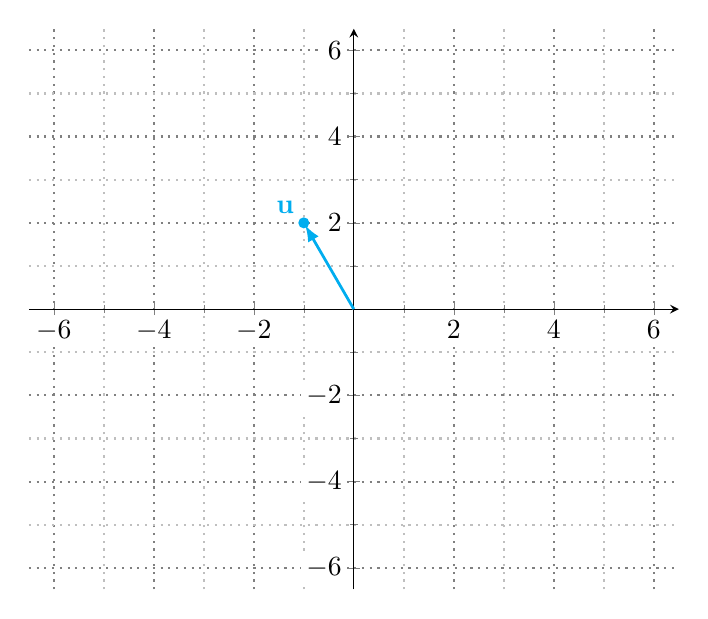
\begin{tikzpicture}
	% Set u and v
	\pgfmathtruncatemacro{\ux}{-1}
	\pgfmathtruncatemacro{\uy}{2}
	% Begin Axis
	\begin{axis}[axis x line=center, axis y line=middle,
	xmin=-6.5, xmax=6.5,
	ymin=-6.5, ymax=6.5,
	xtick={-6,-4,...,6}, ytick={-6,-4,...,6},
	ticklabel style={draw=none, inner sep=2pt, fill=white, text opacity=1},
	scale only axis, width=3.25in,
	grid=both, minor tick num=1,
	major grid style={line width=.8pt, draw=gray, dotted},
	minor grid style={line width=.8pt, draw=gray!50, dotted}]
	% Draw vector
	\draw[-latex, shorten >=.25ex, line width=1pt, cyan] (0,0) -- (\ux,\uy);
	\fill[cyan] (\ux,\uy) circle (2pt) node[above left, fill=white, rounded corners=0.2cm] {$\vect{u}$};
	\end{axis}
	\end{tikzpicture}
	
	\columnbreak
	
	The vector $\vect{u}$ is indicated on the graph to the left. Indicate the following vectors in a similar manner.
	\begin{multicols}{3}
		\begin{enumerate}[(a)]
			\item $\vect{v}$
			\item $-2\vect{u}$
			\item $\vect{u}+\vect{v}$
			\item $\vect{u}-\vect{v}$
			\item $\vect{u}-2\vect{v}$ 
		\end{enumerate}
	\end{multicols}
	\end{multicols}
\end{exercise}


\begin{exercise} % 1.3.5&9
	An augmented matrix for a system is given. For this problem, use the variables $x_1$ and $x_2$.
	$$\begin{bmatrix}
	-2 & 0 & -3 \\ 7 & -7 & 6 \\ 3 & 6 & 5
	\end{bmatrix}$$
	\begin{multicols}{2}
		\begin{enumerate}[(a)]
			\item Rewrite the augmented matrix as a system of linear equations. Do not solve the system.
			\item Rewrite the augmented matrix as a vector equation (using each column as a vector). Do not solve the system.
		\end{enumerate}
	\end{multicols}
	\vfill
	Note that in the first instance, the \textbf{rows} of the matrix are the important objects. In the second instance, we instead view the matrix as a linear combination of the \textbf{columns}.
\end{exercise}


\newpage


\begin{exercise} % 1.3.11
	Determine if $\vect{b}$ is in $\Span\{\vect{a}_1, \vect{a}_2, \vect{a}_3\}$. In other words, determine if $\vect{b}$ can be written as a linear combination of $\vect{a}_1$, $\vect{a}_2$, and $\vect{a}_3$.
	$$ \vect{a}_1 = \begin{bmatrix} 1 \\ -3 \\ 0 \end{bmatrix}, 
	\vect{a}_2 = \begin{bmatrix} 0 \\ 1 \\ 2 \end{bmatrix}, 
	\vect{a}_3 = \begin{bmatrix} 4 \\ -5 \\ 14 \end{bmatrix},
	\vect{b} = \begin{bmatrix} 4 \\ -1 \\ 22 \end{bmatrix}$$
\end{exercise}
\vfill


\begin{exercise} % 1.3.Custom
	For any nonzero vector $\vect{u}$ in $\R^2$, $\Span\{\vect{u}\}$ is a line passing through $\vect{u}$ and the origin, $\vect{0}$. See the picture.
	\begin{multicols}{2}
		\begin{center}
		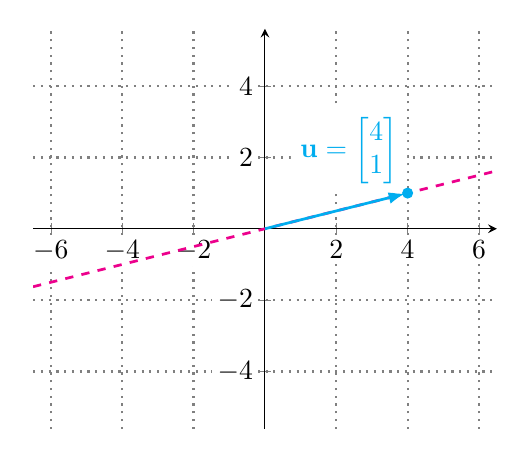
\begin{tikzpicture}
		% Set u
		\pgfmathsetmacro{\ux}{4}
		\pgfmathsetmacro{\uy}{1}
		% Begin Axis
		\begin{axis}[axis x line=center, axis y line=middle,
		xmin=-6.5, xmax=6.5,
		ymin=-3.5, ymax=3.5,
		%		xtick={-6,...,6}, ytick={-3,...,3},
		ticklabel style={draw=none, inner sep=2pt, fill=white, text opacity=1},
		scale only axis, axis equal, height=2in,
		grid=major, grid style={line width=.8pt, draw=gray, dotted}]
		% Plot line
		\addplot[-,dashed, magenta, line width=1pt, domain=-6.5:6.5] {(\uy/\ux)*x};
		% Draw vector
		\draw[-latex, shorten >=.25ex, line width=1pt, cyan] (0,0) -- (\ux,\uy);
		\fill[cyan] (\ux,\uy) circle (2pt) node[above left, fill=white, rounded corners=0.2cm] {$\vect{u}=\begin{bmatrix} \ux \\ \uy \end{bmatrix}$};
		\end{axis}
		\end{tikzpicture}
		\end{center}
		
		\columnbreak
		
		If $\vect{u}$ and $\vect{v}$ are distinct nonzero vectors in $\R^3$, then $\Span\{\vect{u},\vect{v}\}$ \emph{may} be a plane passing through $\vect{u}$, $\vect{v}$, and $\vect{0}$ (as below)... but this is not always the case!
		\begin{center}
		\includegraphics[width=\linewidth]{img/1_3_Plane}
		\end{center}
	\end{multicols}

	Give an example of two distinct, nonzero vectors $\vect{u}$ and $\vect{v}$ in $\R^3$ so that $\Span\{\vect{u},\vect{v}\}$ is \textbf{not} a plane. What is the geometric interpretation of $\Span\{\vect{u},\vect{v}\}$ for your example?
\end{exercise}
\vspace{1.5in}

\begin{exercise} % locations in a qr code as a vector equation

  Quick response (QR) codes are used to display pixels in a two
  dimensional array. A pixel is either black or white. Smartphone apps
  take an image of a QR code and convert the pixels into a string of
  characters. There are a number of important positions in a QR code
  including the position markers in the lower left, upper left, and
  upper right of the code.

  The markers help identify the orientation of the code. An example of
  the codes is shown in Figure \ref{fig:qrCodeExample}.

  \begin{figure}[h]
    %\centering
    \begin{tabular}[h]{p{5cm}@{\hspace{3em}}p{5cm}}
    \qrcode[nolink,level=L,height=5cm]{abcd} &
     \begin{minipage}[h]{5cm}
         \vspace{1.5em}
         \includegraphics[height=5cm]{img/qrCodeSnapshot}
     \end{minipage}
    \end{tabular}
    \caption{Example of a QR code. The code on the left is the
      original, and the code on the right is the skewed image obtained
      using a mobile phone.}
    \label{fig:qrCodeExample}
  \end{figure}

    \begin{figure}[h]
    \centering
    \begin{tabular}{l@{\hspace{3em}}r}
      \includegraphics[width=6cm]{img/qrCodeSnapshotUV} &
      \includegraphics[width=6cm]{img/qrCodeSnapshotUV-coordinates}
    \end{tabular}
    \caption{Example of a QR code. The code on the left indicates the
      horizontal and vertical directions for the image of the
      code. The code on the right indicates the locations of the
      pixels marking the tail and the head of the vectors indicating
      the directions. }
    \label{fig:qrCodeExampleDirections}
  \end{figure}

  \begin{figure}[h]
    \centering
    %\begin{tabular}{l@{\hspace{3em}}r}
      \includegraphics[width=6cm]{img/qrCodeSnapshotUV-points.png}
    %\end{tabular}
    \caption{Example of a QR code. The pixels indicated by points $a$,
    $b$, $c$ and $d$ are locations that provide information about the
    text for the code. Each location should either be a black square
    or a white square.}
    \label{fig:qrCodeExampleLocations}
  \end{figure}

\end{exercise}


\clearpage
\newpage


% SEC 1.4
\section{The Matrix Equation $\boldsymbol{Ax=b}$}
\sectionmark{The Matrix Equation $A\vect{x}=\vect{b}$}
\name[2.25in]

\begin{exercise} % 1.4.3
	A matrix $A$ and column vector $\vect{x}$ are given.
	\begin{align*}
	A &= \begin{bmatrix}6&5\\-3&-4\\7&4\end{bmatrix}, &
	\vect{x} &= \begin{bmatrix}3\\-2\end{bmatrix}
	\end{align*}
	There are two main ways to think about the product $A\vect{x}$.
	\begin{multicols}{2}
		\begin{enumerate}[(a)]
			\item Write the product $A\vect{x}$ as a linear combinations of the columns of $A$ using the entries of $\vect{x}$ as weights. Compute the product.
			\columnbreak
			\item Compute the product $A\vect{x}$ using the row-vector rule. Show your work clearly. \par
			$ A\vect{x} = \begin{bmatrix}6&5\\-3&-4\\7&4\end{bmatrix}\begin{bmatrix}3\\-2\end{bmatrix} = $
		\end{enumerate}
	\end{multicols}
\end{exercise}
\vfill

\begin{boxthm}
	\textbf{Theorem 3.} \\
	If $A$ is an $m\times n$ matrix with columns $\vect{a}_1,\ldots,\vect{a}_n$, and if $\vect{b}$ is in $\R^m$, the matrix equation $A\vect{x}=\vect{b}$ has the same solutions set as the vector equation $x_1\vect{a}_1+x_2\vect{a}_2+\cdots+x_n\vect{a}_n=\vect{b}$ which, in turn, has the same solution set as the system of linear equations whose augmented matrix is $\begin{bmatrix}\vect{a}_1&\vect{a}_2&\cdots&\vect{a}_n&\vect{b}\end{bmatrix}$.
\end{boxthm}

\begin{exercise} % 1.4.11
	Write the augmented matrix that corresponds to the matrix equation $A\vect{x}=\vect{b}$ and solve the system to find $\vect{x}$.
	\begin{align*}
	A &= \begin{bmatrix}1&2&-4\\1&5&2\\2&3&2\end{bmatrix} &
	\vect{b} &= \begin{bmatrix}-17\\22\\13\end{bmatrix}
	\end{align*}
\end{exercise}
\vfill


\newpage


\begin{boxthm}
	\textbf{Theorem 4.} \\
	Let $A$ be an $m\times n$ matrix. Then the following statements are logically equivalent.
	\begin{enumerate}[(a)]\itemsep0em 
		\item For each $\vect{b}$ in $\R^m$, the equation $A\vect{x}=\vect{b}$ has a solution.
		\item Each $\vect{b}$ in $\R^m$ is a linear combination of the columns of $A$.
		\item The columns of $A$ span $\R^m$.
		\item $A$ has a pivot position in every row.
	\end{enumerate}
\end{boxthm}

\begin{exercise} % 1.4.16
	Show that the equation $A\vect{x}=\vect{b}$ does not have a solution for all possible $\vect{b}$, and describe the set of all $b$ for which $A\vect{x}=\vect{b}$ does have a solution.
	\begin{align*}
	A &= \begin{bmatrix}1&-4&-3\\-3&3&0\\4&2&6\end{bmatrix} &
	\vect{b} &= \begin{bmatrix}b_1\\b_2\\b_3\end{bmatrix}
	\end{align*}
	(Hint: Note that by Theorem 4, to show that $A\vect{x}=\vect{b}$ does not have a solution for all $\vect{b}$, you just need to show that $A$ does not have a pivot in every row. However, to determine $\vect{b}$ for which $A\vect{x}=\vect{b}$ does have a solution, you will need to put the augmented matrix $\begin{bmatrix}\vect{a}_1&\vect{a}_2&\vect{a}_3&\vect{b}\end{bmatrix}$ in row echelon form.)
\end{exercise}
\vfill

\begin{exercise} % 1.4.13
	The columns of the matrix $A$ span a plane in $\R^3$. Is $\vect{u}$ in the plane spanned by the columns of $A$? If so, write $\vect{u}$ as a linear combination of the columns of $A$.
	\begin{align*}
	A &= \begin{bmatrix}4&-6\\-3&5\\1&1\end{bmatrix} &
	\vect{u} &= \begin{bmatrix}6\\-3\\9\end{bmatrix}
	\end{align*}
\end{exercise}
\vfill


\newpage

% SEC 1.5
\section{Solution Sets of Linear Systems}
\name[2in]

\begin{boxme}
	The homogeneous equation $A\vect{x}=\vect{0}$ has a nontrivial solution if, and only if, the equation has at least one free variable.
\end{boxme}
\begin{exercise} % 1.5.3
	Determine if the system has a nontrivial solution.
	$$\systeme{-2x_1+6x_2-6x_3=0,-4x_1+8x_2+3x_3=0}$$
\end{exercise}
\vfill

\begin{boxme}
	\begin{multicols}{2}
	To write a solution set in parametric vector form:
	\begin{enumerate}[(1)]\itemsep0em 
		\item Row reduce augmented matrix to RREF
		\item Express basic var. in terms of free var.
		\item Write the solution $\vect{x}$ as a vector whose entries depend on the free variables.
		\item Decompose $\vect{x}$ into a linear combination of vectors using free variables as parameters.
	\end{enumerate}
	
	\columnbreak
	
	\textbf{Example.}
	Solution set: $\begin{cases}x_1=3-2x_3 \\ x_2 = -4 \\ x_3 \text{ is free}\end{cases}$
	$$\vect{x}=\begin{bmatrix}x_1\\x_2\\x_3\end{bmatrix}
	=\begin{bmatrix}3-2x_3\\-4\\x_3\end{bmatrix}
	=\begin{bmatrix}3\\-4\\0\end{bmatrix} +x_3\begin{bmatrix}-2\\0\\1\end{bmatrix}$$
	\end{multicols}
\end{boxme}
\begin{exercise} % 1.5.7
	The matrix $A$ is given below along with its reduced echelon form and the associated system of equations of the matrix equation $A\vect{x}=\vect{0}$.
	$$A=\begin{bmatrix}1&4&-3&5\\1&5&-5&7\end{bmatrix}\xrightarrow{\text{RREF}}
	\begin{bmatrix}1&0&5&-3\\0&1&-2&2\end{bmatrix}\xrightarrow{\text{System}}
	\systeme{x_1 + 5x_3 - 3x_4 = 0, x_2 - 2x_3 + 2x_4 = 0} $$
	\begin{enumerate}[(a)]
		\item Describe the solution set of $\Axz$ in parametric vector form.
		\vfill
		\item Circle the best answer. \par
		The solution set of $A\vect{x}=\vect{0}$ is a: \quad \textbf{Single Vector} \qquad \textbf{Line} \qquad \textbf{Plane} \qquad \textbf{None of these}
	\end{enumerate}
\end{exercise}


\newpage


\begin{exercise} % 1.5.15
	\textbf{Compare $\Axb$ and $\Axz$} \par
	The solution sets of the systems of linear equations below are given.
	
	\noindent	
	\begin{tabular}{c|c}
		\parbox{0.5\linewidth}{%
			\begin{align*}
			\systeme{2x_1+2x_2+4x_3=8,-4x_1-4x_2-8x_3=-16,-3x_2+6x_3=9}&&
			\begin{cases}x_1 = 7-4x_3 \\ x_2 =-3+2x_3 \\ x_3 \text{ is free}\end{cases}
			\end{align*}}
		&
		\parbox{0.5\linewidth}{%
			\begin{align*}
			\systeme{2x_1+2x_2+4x_3=0,-4x_1-4x_2-8x_3=0,-3x_2+6x_3=0}&&
			\begin{cases}x_1 = -4x_3 \\ x_2 =2x_3 \\ x_3 \text{ is free}\end{cases}
			\end{align*}}
	\end{tabular}
	
	\begin{enumerate}[(a)]
		\item Write the solution sets in parametric vector form.
		\begin{multicols}{2}
			\begin{enumerate}[(i)]
				\item First System
				\item Second System
			\end{enumerate}
		\end{multicols}
		\vfill
		\item Provide a geometric comparison between the solution sets of the two systems. (Are the solution sets single vectors? Lines? Planes? Something else? How are they related to one another?)
		\vspace{1in}
	\end{enumerate}
\end{exercise}

\begin{exercise} % 1.5.
	A $3\times 4$ matrix $A$ has 3 pivot positions.
%	e.g.
%	$\begin{bmatrix}
%	\blacksquare	& *	& 0				& *				& * \\ 
%	0				& 0	& \blacksquare	& * 			& * \\ 
%	0				& 0	& 0				& \blacksquare	& *
%	\end{bmatrix}$
	\begin{multicols}{2}
		\begin{enumerate}[(a)]
			\item Does the equation $\Axz$ have a nontrivial solution? How do you know?
			\item Does the equation $\Axb$ have at least one solution for any choice of $\vect{b}$ in $\R^3$? How do you know?
		\end{enumerate}
	\end{multicols}
\end{exercise}
\vfill


\newpage


% SEC 1.6
\section{Applications of Linear Systems}
\names[4]


\begin{exercise} % 1.6.3 textbook
	Consider an economy with 3 sectors, Chemicals \& Metals, Fuels \& Power, and Machinery. Chemicals sells 30\% of its output to Fuels and 50\% to Machinery and retains the rest. Fuels sells 80\% of its output to Chemicals and 10\% to Machinery and retains the rest. Machinery sells 40\% to Chemicals and 40\% to Fuels and retains the rest.
	\begin{enumerate}[(a)]
		\item Construct the exchange table for this economy. \par
			\renewcommand{\arraystretch}{2}
			\begin{tabular}{|c|c|c|c|}
				\hline
				\textbf{Chem}	& \textbf{Fuels}	& \textbf{Mach}	& \textbf{Purchased by:} \\ \hline
				&	&	& Chem \\ \hline
				&	&	& Fuel \\ \hline
				&	&	& Mach \\ \hline
			\end{tabular}
		\item Develop a system of equations that leads to prices at which each sector's income matches its expenses using $p_C$, $p_F$, and $p_M$ for the price of Chemicals, Fuels, and Machinery outputs, respectively. Then write the augmented matrix that can be row reduced to find these prices.
		\vfill
		\item Find a set of equilibrium prices when the price for the Machinery ouput is 100 units.
		\vfill
	\end{enumerate}
\end{exercise}


\newpage


\begin{exercise} % 1.6.7
	Alka-Seltzer contains sodium bicarbonate (\ce{NaHCO3}) and citric acid (\ce{H3C6H5O7}). When a tablet is dissolved in water, the following reaction produces sodium citrate, water, and carbon dioxide (gas):
	\begin{center}
		\ce{NaHCO3 + H3C6H5O7 -> Na3C6H5O7 + H2O + CO2} \\
		%\ce{3NaHCO3 + 1H3C6H5O7 -> 1Na3C6H5O7 + 3H2O + 3CO2}
	\end{center}
	Balance the chemical equation. (Hint: there are 5 unknowns---one for each of the 5 molecules. The column vectors you construct will each contain 4 entries---one for each type of atom present, Na, H, C, and O)
\end{exercise}
\vfill

%\begin{exercise} % 1.6.9
%	Balance the chemical equation. Assume the coefficient of NO is 90.
%	\begin{center}
%		\ce{PbN6 + CrMn2O8 -> Pb3O4 + Cr2O3 + MnO2 + NO}
%		%\ce{15PbN6 + 44CrMn2O8 -> 5Pb3O4 + 22Cr2O3 + 88MnO2 + 90NO}
%	\end{center}
%\end{exercise}
%\vfill


\begin{exercise} % 1.6.11
	\begin{enumerate}[(a)]
		\item Find the general flow pattern of the network shown in the figure. \par
		% ADD IN TABLE FOR FLOW IN & OUT OF EACH NODE
			\hfill
			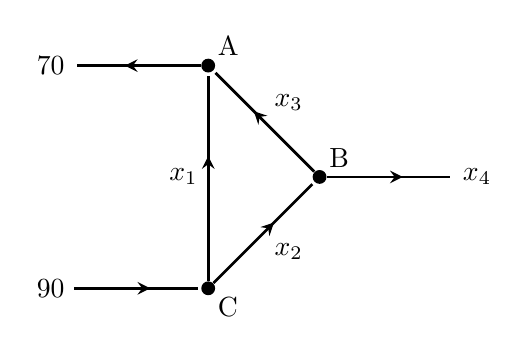
\begin{tikzpicture}[shorten >=1pt,node distance=2cm,on grid,auto]
			\tikzset{->-/.style={decoration={markings,mark=at position .6 with {\arrow{stealth}}},postaction={decorate}}}
			\tikzstyle{every edge}=[draw,->-,line width=1pt]
			\tikzset{junction/.style={fill=black,draw=none,inner sep=0pt, minimum size=5pt,circle}}
			% Place Nodes
			\node (OUT1) {70};
			\node[junction] (A) [right=of OUT1] {};
			\node[junction] (B) [below right=of A] {};
			\node[junction] (C) [below left=of B] {};
			\node (IN) [left=of C] {90};
			\node (OUT2) [right=of B] {$x_4$};
			% Label nodes
			\draw (A) node[above right] {A};
			\draw (B) node[above right] {B};
			\draw (C) node[below right] {C};
			% Draw flow paths
			\path
			(A) edge (OUT1)
			(B) edge node[above right] {$x_3$} (A)
			(B) edge (OUT2)
			(C) edge node[below right] {$x_2$} (B)
			(C) edge node {$x_1$} (A)
			(IN) edge (C);
			\end{tikzpicture}
		\vfill
		\item Assuming that the flows are all nonnegative, what is the largest possible value for $x_3$?
		\vspace{2em}
	\end{enumerate}
% Solution
%$\begin{cases}
%	x_1 = 70 - x_3 \\
%	x_2 = 20 + x_3 \\
%	x_3 \text{ is free} \\
%	x_4 = 20
%	\end{cases}$
\end{exercise}


\newpage


% SEC 1.7
\section{Linear Independence}
\name

\begin{boxdef}
	An indexed set of vectors $\{\vect{v}_1,\ldots,\vect{v}_p\}$ in $\R^n$ is said to be \textbf{linearly independent} if the vector equation
	$$ x_1\vect{v}_1 + x_2\vect{v}_2 + \cdots + x_p\vect{v}_p = \vect{0} $$
	has only the trivial solution. The set $\{\vect{v}_1,\ldots,\vect{v}_p\}$ is said to be \textbf{linearly dependent} if there exist weights $c_1,\ldots,c_p$ not all zero, such that
	\begin{align*}
	c_1\vect{v}_1 + c_2\vect{v}_2 + \cdots + c_p\vect{v}_p = \vect{0}. \tag{\dag}
	\end{align*}
	The equation $(\dag)$ is called a \textbf{linear dependence relation}. (Note that each linear dependence relation corresponds to a nontrivial solution of the vector equation.)
\end{boxdef}

\begin{exercise} % 1.7.
	Determine by inspection if the given vectors are linearly independent. If they are not, write a linear dependence relation to prove they are linearly dependent.
	\begin{multicols}{2}
		\begin{enumerate}[(a)]
			\item $$\vect{u}=\begin{bmatrix}3\\-2\end{bmatrix}, \vect{v}=\begin{bmatrix}-9\\6\end{bmatrix}$$
			\item $$\vect{w}=\begin{bmatrix}0\\0\\0\\0\end{bmatrix}, \vect{z}=\begin{bmatrix}3\\3\\3\\3\end{bmatrix}$$
		\end{enumerate}
	\end{multicols}
\end{exercise}
\vfill


\begin{boxdef}
	The columns of a matrix $A$ are linearly independent if, and only if, the equation $\Axz$ has \emph{only} the trivial solution.
\end{boxdef}
\begin{exercise} % 1.7.5
	A matrix is given along with its reduced echelon form. Determine if the columns of the matrix are linearly independent. Explain your answer.
	\begin{multicols}{2}
		\begin{enumerate}[(a)]
			\item
				\begin{align*}
				A = \begin{bmatrix}0&-3&9\\2&1&-7\\-1&4&-4\\1&-4&-2\end{bmatrix}
				&\xrightarrow{\text{RREF}}
				\begin{bmatrix}1&0&0\\0&1&0\\0&0&1\\0&0&0\end{bmatrix}
				\end{align*}
			\item 
				\begin{align*}
				B = \begin{bmatrix}1&-3&5&0\\3&-9&6&1\\2&-6&0&1\end{bmatrix}
				&\xrightarrow{\text{RREF}}
				\begin{bmatrix}1&-3&0&0\\0&0&1&0\\0&0&0&1\end{bmatrix}
				\end{align*}
		\end{enumerate}
	\end{multicols}
\end{exercise}
\vfill


\newpage


\begin{exercise} % 1.7.31
	Given $A=\begin{bmatrix}2&4&6\\-6&1&-5\\-4&-2&-6\\4&0&4\end{bmatrix}$, observe that the 3rd column is the sum of the 1st and 2nd columns.
		\begin{enumerate}[(a)]
			\item Without performing row operations, give a nontrivial solution of $\Axz$.
			\vfill
			\item Write $A\vect{x}$ as a linear combination of the columns of $A$ using the entries of your solution to part (a) as weights. Simplify the expression to show that your solution to part (a) is correct.
			\vfill
		\end{enumerate}
\end{exercise}


\begin{boxthm}
	\textbf{Theorem 7.}
	\textbf{Characterization of Linearly Independent Sets (Short Version)} \\
	An indexed set $S=\{\vect{v}_1,\ldots,\vect{v}_p\}$ of two or more vectors is linearly dependent if, and only if, at least one of the vectors in $S$ is a linear combination of the others.
\end{boxthm}
\begin{boxthm}
	\textbf{Theorem 8.} \\
	If a set contains more vectors than there are entries in each vector, then the set is linearly dependent. That is, any set $\{\vect{v}_1,\ldots,\vect{v}_p\}$ in $\R^n$ is linearly dependent if $p>n$.
\end{boxthm}
\begin{exercise} % 1.7.Custom
	Determine if the following vectors are linearly independent or linearly dependent. Explain your answer. Be sure to reference the appropriate theorem.
		\begin{multicols}{2}
			\begin{enumerate}[(a)]
				\item
					$$
					\begin{bmatrix} 2\\1\\-5 \end{bmatrix},
					\begin{bmatrix} 5\\-7\\3 \end{bmatrix},
					\begin{bmatrix} -6\\-3\\15 \end{bmatrix}
					$$
					Circle one and explain your answer:
					\begin{center}
						\shortstack{\textbf{Linearly}\\ \textbf{Independent}} \qquad
						\shortstack{\textbf{Linearly}\\ \textbf{Dependent}}
					\end{center}
				
				\columnbreak
				
				\item
					$$
					\begin{bmatrix}  2\\ 3\\ 5\\ 7 \end{bmatrix},
					\begin{bmatrix} 11\\13\\17\\19 \end{bmatrix},
					\begin{bmatrix} 23\\29\\31\\37 \end{bmatrix},
					\begin{bmatrix} 41\\43\\47\\53 \end{bmatrix},
					\begin{bmatrix} 59\\61\\67\\71 \end{bmatrix}
					$$
					Circle one and explain your answer:
					\begin{center}
						\shortstack{\textbf{Linearly}\\ \textbf{Independent}} \qquad
						\shortstack{\textbf{Linearly}\\ \textbf{Dependent}}
					\end{center}
			\end{enumerate}
		\end{multicols}
\end{exercise}
\vfill


%\begin{exercise} % 1.7.Custom
%	If you have a linearly independent set of vectors, $\{\vect{u},\vect{v}\}$ and you know that $\vect{w}$ is in $\Span\{\vect{u},\vect{v}\}$, can you determine whether the set $\{\vect{u},\vect{v},\vect{w}\}$ is linearly independent or not?
%\end{exercise}
%\vfill


\newpage


% SEC 1.8
\section[Introduction to Linear Transformations]{Intro to Linear Transformations}
\name[2in]

\begin{boxdef}
	A \textbf{transformation} $T:\R^n\to\R^m$ is a rule that assigns to each vector in $\R^n$ a vector $T(\vect{x})$ in $\R^m$. The set $\R^n$ is called the \textbf{domain} of $T$, and $\R^m$ is called the \textbf{codomain} of $T$. For $\vect{x}\in\R^n$, the vector $T(\vect{x})$ is called the \textbf{image} of $\vect{x}$ (under the action of $T$). The set of all images $T(\vect{x})$ is called the \textbf{range} of $T$.
\end{boxdef}

\begin{exercise} % 1.8.Custom
	Suppose we define a transformation $T$ by $T(\vect{x})=\Ax$ where $A=\begin{bmatrix}1&3&1\\2&6&8\\0&0&0\\0&0&1\end{bmatrix}$.
	\begin{enumerate}[(a)]
		\item What is the domain of $T$?
		\vspace{1em}
		\item What is the codomain of $T$?
		\vspace{1em}
		\item Are the range and codomain of $T$ the same? Why or why not? \par
		Hint: think of the range as all possible linear combinations of the columns of $A$.
	\end{enumerate}
\end{exercise}
\vfill



\begin{exercise} % 1.8.9
	Find all $\vect{x}$ in $\R^4$ that are mapped into the zero vector by the transformation $\vect{x}\mapsto\Ax$ for the given matrix $A$.
	$$ \begin{bmatrix} 1&-5&18&-3 \\ 0&1&-5&2 \\ 4&-16&52&-4 \end{bmatrix}$$
	% Solution
	%$$ x_3\begin{bmatrix}7\\5\\1\\0\end{bmatrix} + x_4\begin{bmatrix}-7\\-2\\0\\1\end{bmatrix}$$
\end{exercise}
\vfill


\newpage


\begin{boxme}
	A transformation $T$ is \textbf{linear} if:
	\begin{enumerate}[(i)]\itemsep=0pt
		\item $T(\vect{u}+\vect{v}) = T(\vect{u})+T(\vect{v})$ for all $\vect{u},\vect{v}$ in the domain of $T$.
		\item $T(c\vect{u}) = cT(\vect{u})$ for all scalars $c$ and all $\vect{u}$ in the domain of $T$.
	\end{enumerate}
	This implies the following:
	\begin{enumerate}[(i)]\itemsep=0pt
		\item $T(\vect{0})=\vect{0}.$
		\item $T(c\vect{u}+d\vect{v}) = cT(\vect{u})+dT(\vect{v})$ for all scalars $c,d$ and all vectors  $\vect{u},\vect{v}$ in the domain of $T$.
	\end{enumerate}
	Note: to prove a transformation $T$ is linear, you only need to show $T(c\vect{u}+d\vect{v}) = cT(\vect{u})+dT(\vect{v})$.
\end{boxme}

\begin{exercise} % 1.8.17
	A linear transformation $T:\R^2\to\R^2$ maps the vector $\vect{u}=\begin{bmatrix}6\\3\end{bmatrix}$ to $\begin{bmatrix}5\\1\end{bmatrix}$ and maps the vector $\vect{v}=\begin{bmatrix}3\\3\end{bmatrix}$ to $\begin{bmatrix}-1\\3\end{bmatrix}$. Use that fact that $T$ is linear to find the image of $3\vect{u}+4\vect{v}$ under $T$.
\end{exercise}
\vfill


\begin{exercise} % 1.8.15
	The vectors $\vect{u}=\begin{bmatrix}-2\\5\end{bmatrix}$ and $\vect{v}=\begin{bmatrix}3\\-1\end{bmatrix}$ are plotted on the graph below.
	\begin{enumerate}[(a)]
		\item Plot $T(\vect{u})$ and $T(\vect{v})$ under the given transformation $T$.
		
		$$ \Tx = \begin{bmatrix}1&0\\0&0\end{bmatrix}\begin{bmatrix}x_1\\x_2\end{bmatrix} $$
		
		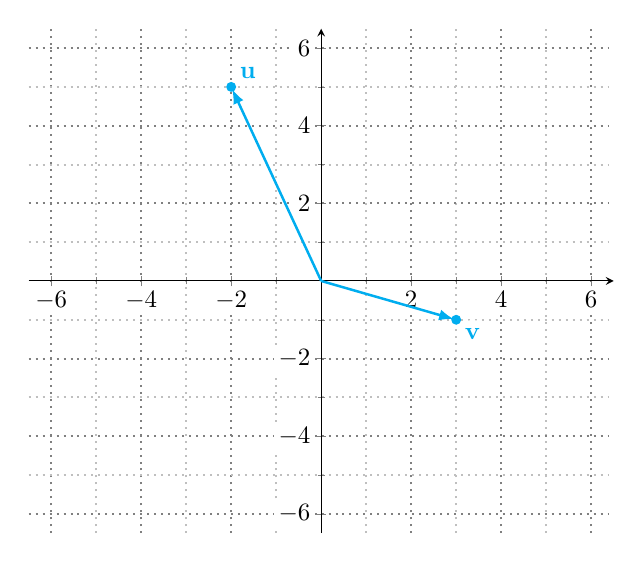
\begin{tikzpicture}[scale=.9]
		% Set u and v
		\pgfmathtruncatemacro{\ux}{-2}
		\pgfmathtruncatemacro{\uy}{5}
		\pgfmathtruncatemacro{\vx}{3}
		\pgfmathtruncatemacro{\vy}{-1}
		% Begin Axis
		\begin{axis}[axis x line=center, axis y line=middle,
		xmin=-6.5, xmax=6.5,
		ymin=-6.5, ymax=6.5,
		xtick={-6,-4,...,6}, ytick={-6,-4,...,6},
		ticklabel style={draw=none, inner sep=2pt, fill=white, text opacity=1},
		scale only axis, width=3.25in,
		grid=both, minor tick num=1,
		major grid style={line width=.8pt, draw=gray, dotted},
		minor grid style={line width=.8pt, draw=gray!50, dotted}]
		% Draw vectors
		\draw[-latex, shorten >=.25ex, line width=1pt, cyan] (0,0) -- (\ux,\uy);
		\fill[cyan] (\ux,\uy) circle (2pt) node[above right, fill=white, rounded corners=0.2cm] {$\vect{u}$};
		\draw[-latex, shorten >=.25ex, line width=1pt, cyan] (0,0) -- (\vx,\vy);
		\fill[cyan] (\vx,\vy) circle (2pt) node[below right, fill=white, rounded corners=0.2cm] {$\vect{v}$};
		\end{axis}
		\end{tikzpicture}
		
		\item Describe geometrically what $T$ does to each vector $\vect{x}$ in $\R^2$. (Is it a rotation? Reflection? Projection? Shear? Dilation? Contraction? Something else?)
	\end{enumerate}
\end{exercise}
\vspace{2em}


\newpage


% SEC 1.9
\section[The Matrix of a Linear Transformation]{Matrix of a Linear Transformation}
\name[2in]

\begin{boxthm}
	\textbf{Theorem 10.} \\
	Let $T:\R^n\to\R^m$ be a linear transformation. Then there exists a unique matrix $A$ such that $\Tx=\Ax$ for all $\vect{x}$ in $\R^n$. In fact, $A$ is the $m\times n$ matrix whose $j$th column is the vector $\Te{j}$, where $\ve{j}$ is the $j$th column of the identity matrix in $\R^n$:
	$$ A = \begin{bmatrix}\Te1 & \cdots & \Te{n}\end{bmatrix}. $$
\end{boxthm}

\begin{exercise} % 1.9.2
	Suppose $\Tmap{3}{2}$ is a linear transformation such that $\Te1=(1,3)$, $\Te2=(-5,3)$, and $\Te3=(3,-8)$, where $\ve1$, $\ve2$, and $\ve3$ are the columns of the $3\times 3$ identity matrix, $I_3=\begin{bmatrix}1&0&0\\0&1&0\\0&0&1\end{bmatrix}$. Find the standard matrix of $T$.
\end{exercise}
\vfill


\begin{exercise} % 1.9.13
	Let $\Tmap{2}{2}$ be a linear transformation such that $\Te1$ and $\Te2$ are the vectors shown in the figure.
	
	\begin{multicols}{2}
		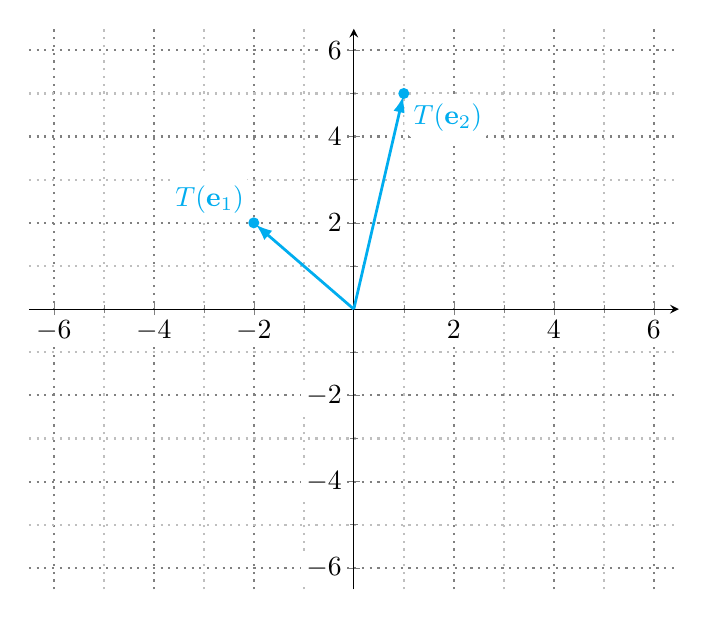
\begin{tikzpicture}[scale=1]
		% Set u and v
		\pgfmathtruncatemacro{\ux}{-2}
		\pgfmathtruncatemacro{\uy}{2}
		\pgfmathtruncatemacro{\vx}{1}
		\pgfmathtruncatemacro{\vy}{5}
		% Begin Axis
		\begin{axis}[axis x line=center, axis y line=middle,
		xmin=-6.5, xmax=6.5,
		ymin=-6.5, ymax=6.5,
		xtick={-6,-4,...,6}, ytick={-6,-4,...,6},
		ticklabel style={draw=none, inner sep=2pt, fill=white, text opacity=1},
		scale only axis, width=3.25in,
		grid=both, minor tick num=1,
		major grid style={line width=.8pt, draw=gray, dotted},
		minor grid style={line width=.8pt, draw=gray!50, dotted}]
		% Draw vectors
		\draw[-latex, shorten >=.25ex, line width=1pt, cyan] (0,0) -- (\ux,\uy);
		\fill[cyan] (\ux,\uy) circle (2pt) node[above left, fill=white, rounded corners=0.2cm] {$\Te1$};
		\draw[-latex, shorten >=.25ex, line width=1pt, cyan] (0,0) -- (\vx,\vy);
		\fill[cyan] (\vx,\vy) circle (2pt) node[below right, fill=white, rounded corners=0.2cm] {$\Te2$};
		\end{axis}
		\end{tikzpicture}
		
		\columnbreak
		
		\begin{enumerate}[(a)]
			\item Using the figure, sketch the vector $T(-2,1)$.
			\vspace{1in}
			\item Write the standard matrix for the linear transformation.
			
				\begin{align*}
				A &=	\huge\begin{bmatrix}
						\phantom{-2}	& \phantom{2} \\
						\phantom{1}		& \phantom{5} \\
						\end{bmatrix}
				\end{align*}
		\end{enumerate}
	\end{multicols}
\end{exercise}


\newpage


\begin{boxdef}
	A mapping $\Tmap{n}{m}$ is said to be \textbf{onto} $\R^m$ if each $\vect{b}$ in $\R^m$ is the image of \emph{at least one} $\vect{x}$ in $\R^n$. The mapping is said to be \textbf{one-to-one} if each $\vect{b}$ in $\R^m$ is the image of \emph{at most one} $\vect{x}$ in $\R^n$.
\end{boxdef}

\begin{boxthm}
	\textbf{Theorem 12.} \\
	Let $T:\R^n\to\R^m$ be a linear transformation, and let $A$ be the standard matrix for $T$. Then:
	\begin{enumerate}[(a)]
		\item $T$ maps $\R^n$ onto $\R^m$ if, and only if, the columns of $A$ span $\R^m$;
		\item $T$ is one-to-one if, and only if, the columns of $A$ are linearly independent.
	\end{enumerate}
\end{boxthm}

\begin{exercise} % 1.9.Custom
	A linear transformation $\Tmap{4}{3}$ has standard matrix $A$. The reduced row echelon form of $A$ is given below.
	$$\begin{bmatrix}1&0&-5&0\\0&1&2&0\\0&0&0&1\end{bmatrix}$$
	\begin{multicols}{2}
		\begin{enumerate}[(a)]
			\item Is $T$ one-to-one? Explain.
			\item Does $T$ map $\R^4$ onto $\R^3$? Explain.
		\end{enumerate}
	\end{multicols}
\end{exercise}
\vfill


\begin{exercise} % 1.9.7
	The standard matrix for rotation about the origin by an angle $\theta$ is $A=\RotMat$. This is because the transformation affects $\ve1$ and $\ve2$ in the following way:
	\begin{align*}
	\begin{bmatrix}1\\0\end{bmatrix} &\mapsto
	\begin{bmatrix} \cos\theta\\ \sin\theta \end{bmatrix} &
	\begin{bmatrix}0\\1\end{bmatrix} &\mapsto
	\begin{bmatrix} -\sin\theta\\ \cos\theta \end{bmatrix}.
	\end{align*}
	Find the standard matrix for the transformation that rotates points by $\frac{\pi}{3}$ radians and then reflects them over the horizontal $x_1$-axis. Simplify any trigonometric expressions.
\end{exercise}
\vfill


\newpage




% CH 2
\chapter{Matrix Algebra}
\chaptermark{Matrix Algebra}

% SEC 2.1
\section{Matrix Operations}
\name

Use the following matrices for the problems on this page.
\begin{align*}
A &= \begin{bmatrix}3&0&-2\\4&-5&3\end{bmatrix} &
B &= \begin{bmatrix}7&-4&2\\2&-3&-2\end{bmatrix} &
C &= \begin{bmatrix}2&3\\-3&2\end{bmatrix} &
D &= \begin{bmatrix}3&6\\-2&3\end{bmatrix} &
E &= \begin{bmatrix}-6\\3\end{bmatrix}
\end{align*}

\begin{exercise} % 2.1.2
	Compute the matrix sum or explain why the expression is undefined.
	\begin{multicols}{2}
		\begin{enumerate}[(a)]
			\item $A+2B$
			\item $4C-2E$
		\end{enumerate}
	\end{multicols}
\end{exercise}
\vfill


\begin{exercise} % 2.1.2
	Compute the matrix product or explain why the expression is undefined.
	\begin{multicols}{2}
		\begin{enumerate}[(a)]
			\item $EB$
			\item $DB$
		\end{enumerate}
	\end{multicols}
\end{exercise}
\vfill


\newpage


\begin{boxme}
	If $A$ is an $m\times n$ matrix and $B=\begin{bmatrix}\vect{b}_1&\vect{b}_2&\cdots&\vect{b}_p\end{bmatrix}$ is an $n\times p$ matrix, then the product $AB$ is the $m\times p$ matrix
	$$ AB = \begin{bmatrix}A\vect{b}_1&A\vect{b}_2&\cdots&A\vect{b}_p\end{bmatrix}. $$
	In other words, each column of $AB$ is a linear combination of the columns of $A$ using the entries of the corresponding columns of $B$ as weights.
\end{boxme}
\begin{exercise} % 2.1.5
	Let $A$ and $B$ be as below. Denote the first and second columns of $B$ by $\vect{b}_1$ and $\vect{b}_2$, respectively.
	\begin{align*}
	A &= \begin{bmatrix}-1&4\\2&5\\5&-2\end{bmatrix} &
	B &= \begin{bmatrix}4&-2\\-3&3\end{bmatrix}
	\end{align*}
	\begin{multicols}{2}
		\begin{enumerate}[(a)]
			\item Compute $A\vect{b}_1$ and $A\vect{b_2}$.
			\begin{align*}
			A\vect{b}_1 &=
			\begin{bmatrix}-1&4\\2&5\\5&-2\end{bmatrix}
			\begin{bmatrix}4\\-3\end{bmatrix}
			= 4\begin{bmatrix}-1\\2\\5\end{bmatrix}
			-3\begin{bmatrix}4\\5\\-2\end{bmatrix} \\
			&=
%			\begin{bmatrix}-4\\8\\20\end{bmatrix} +
%			\begin{bmatrix}-12\\-15\\6\end{bmatrix} =
%			\begin{bmatrix}-16\\-7\\26\end{bmatrix}
			\begin{bmatrix}\phantom{--}\\{}\\{}\\{}\end{bmatrix} +
			\begin{bmatrix}\phantom{--}\\{}\\{}\\{}\end{bmatrix} = \begin{bmatrix}\phantom{--}\\{}\\{}\\{}\end{bmatrix}\\ \\ \\
			A\vect{b}_2 &=
			\end{align*}
			\item Using part (a), write the matrix $AB$.
		\end{enumerate}
	\end{multicols}
\end{exercise}
\vfill


\begin{exercise} % 2.1.12
	Let $A=\begin{bmatrix}4&-8\\-4&8\end{bmatrix}$. Construct a $2\times 2$ matrix $B$ such that $AB$ is the zero matrix. Use two different columns for $B$.
\end{exercise}
\vfill


\newpage


% SEC 2.2
\section{The Inverse of a Matrix}
\name


\begin{boxdef}
	If $A$ is a matrix, the unique inverse of $A$, denoted $A^{-1}$, is defined so that $A^{-1}A=I$ and $AA^{-1}=I$.
\end{boxdef}
\vspace{-1em}

\begin{boxthm}
	\textbf{Theorem 4. (For $2\times 2$ Matrices)} \\
	Let $A=\begin{bmatrix}a&b\\c&d\end{bmatrix}$. If $ad-bc\neq 0$, then $A$ is invertible and
	$ A^{-1} = \frac{1}{ad-bc}\begin{bmatrix}d&-b\\-c&a\end{bmatrix}.$ \par
	If $ad-bc=0$, then $A$ is not invertible.
\end{boxthm}

\begin{exercise} % 2.2.1
	Determine if the matrix is invertible by checking to see that $ad-bc\neq 0$. If the matrix is invertible, use Theorem 4 to find the inverse.
	\begin{multicols}{2}
		\begin{enumerate}[(a)]
			\item $$A=\begin{bmatrix}9&4\\5&2\end{bmatrix}$$
			Circle one. If $A$ is invertible, find $A^{-1}$.
			\begin{center}
				\shortstack{\textbf{Invertible}} \hspace{5em}
				\shortstack{\textbf{Not}\\ \textbf{Invertible}}
			\end{center}
			
			\item $$B=\begin{bmatrix}6&-9\\-2&3\end{bmatrix}$$
			Circle one. If $B$ is invertible, find $B^{-1}$.
			\begin{center}
				\shortstack{\textbf{Invertible}} \hspace{5em}
				\shortstack{\textbf{Not}\\ \textbf{Invertible}}
			\end{center}
		\end{enumerate}
	\end{multicols}
\end{exercise}
\vfill


\begin{boxthm}
	\textbf{Theorem 5.} \\
	If $A$ is an invertible $n\times n$ matrix, then for each $\vect{b}$ in $\R^n$, the equation $\Axb$ has the unique solution $\vect{x}=A^{-1}\vect{b}$.
\end{boxthm}

\begin{exercise} % 2.2.7
	Suppose $A$ is an invertible $2\times 2$ matrix with inverse $A^{-1}=\begin{bmatrix}3&2\\6&5\end{bmatrix}$, and let $\vect{b}=\begin{bmatrix}2\\-1\end{bmatrix}$.
	\begin{enumerate}[(a)]
		\item Use Theorem 5 to solve the equation $\Axb$.
		\vfill
		\item Suppose $A$ is the standard matrix for a linear transformation $\Tmap{2}{2}$. Is $T$ one-to-one? Explain. \par
		(It may be helpful to consider Theorem 7 on the next page and Theorem 12 from section 1.9).
		\vspace{2em}
	\end{enumerate}
\end{exercise}


\newpage


\begin{boxthm}
	\textbf{Theorem 7.} \\
	An $n\times n$ matrix $A$ is invertible if, and only if, $A$ is row equivalent to $I_n$, and in this case, any sequence of elementary row operations that reduces $A$ to $I_n$ also transforms $I_n$ into $A^{-1}$.
\end{boxthm}
\begin{boxdef}
	Row reduce the augmented matrix $\begin{bmatrix}A&I\end{bmatrix}$. If $A$ is row equivalent to $I$, then $\begin{bmatrix}A&I\end{bmatrix}$ is row equivalent to $\begin{bmatrix}I&A^{-1}\end{bmatrix}$. Otherwise, $A$ does not have an inverse.
\end{boxdef}


\begin{exercise} % 2.2.31
	Find the inverse of $A$, if it exists.
	$$ A = \begin{bmatrix}1&0&4\\-3&1&-2\\2&3&-2\end{bmatrix} $$
	Use Theorem 7 and the proceeding comment, i.e., row reduce the following matrix:\par
	\vspace{1em}
	$\begin{bmatrix}A&I\end{bmatrix} = 
	\begin{amatrix}{3}{3}
		1&0&4&1&0&0\\
		-3&1&-2&0&1&0\\
		2&3&-2&0&0&1
	\end{amatrix}$
%	$\begin{amatrix}{3}{3}
%		-\frac{1}{10}	&-\frac{3}{10}	&\frac{1}{10}	&1&0&0\\
%		\frac{1}{4}		&\frac{1}{4}	&\frac{1}{4}	&0&1&0\\
%		\frac{11}{40}	&\frac{3}{40}	&-\frac{1}{40}	&0&0&1
%		\end{amatrix}$
\end{exercise}
\vfill


\begin{exercise} % 2.2.37
	Let $A=\begin{bmatrix}1&2\\1&3\\1&5\end{bmatrix}$ and $C=\begin{bmatrix}1&1&-1\\-1&1&0\end{bmatrix}$.
	\begin{enumerate}[(a)]
		\item Show that $CA=I_2$.
		\vfill
		\item Is $C$ the inverse of $A$? Why or why not?
		\vspace{2em}
	\end{enumerate}
\end{exercise}


\newpage


% SEC 2.3
\section{Characterizations of Invertible Matrices}
\name[1.5in]

\begin{boxthm}
	\textbf{Theorem 2.8.}
	\textbf{The Invertible Matrix Theorem} \\
	Let $A$ be a square $n\times n$ matrix. Then the following statements are equivalent. That is, for a given $A$, the statements are either all true or all false.
	\begin{enumerate}[(a)]\itemsep0em 
		\item $A$ is an invertible matrix.
		\item $A$ is row equivalent to the $n\times n$ identity matrix.
		\item $A$ has $n$ pivot positions.
		\item The equation $\Axz$ has only the trivial solution.
		\item The columns of $A$ form a linearly independent set.
		\item The linear transformation $\vect{x}\mapsto\Ax$ is one-to-one.
		\item The equation $\Axb$ has at least one solution for each $\vect{b}$ in $\R^n$.
		\item The columns of $A$ span $\R^n$.
		\item The linear transformation $\vect{x}\mapsto\Ax$ maps $\R^n$ onto $\R^n$.
		\item There is an $n\times n$ matrix $C$ such that $CA=I$.
		\item There is an $n\times n$ matrix $D$ such that $AD=I$.
		\item $A^T$ is an invertible matrix.
	\end{enumerate}
\end{boxthm}

\begin{exercise} % 2.3.1-8 Custom
	Using as few calculations as possible, determine which of the following matrices are invertible. Explain your reasoning.
	\begin{enumerate}[(a)]
		\item $\begin{bmatrix}0&1\\-1&0\end{bmatrix}$ \vfill\hrule\vfill
		\item $\begin{bmatrix}5&13\\2&5\end{bmatrix}$ \vfill\hrule\vfill
		\item $\begin{bmatrix}-10&0\\15&0\end{bmatrix}$ \vfill\hrule\vfill
		\item $\begin{bmatrix}1&5&8&10\\0&2&6&9\\0&0&3&7\\0&0&0&4\end{bmatrix}$ \vfill\hrule\vfill
		\item $\begin{bmatrix}-1&3&2\\2&0&5\\3&-9&-6\end{bmatrix}$ \vfill\hrule\vfill
		\item $\begin{bmatrix}2&0&0\\-5&2&0\\11&-4&-2\end{bmatrix}$ \vfill
	\end{enumerate}
\end{exercise}


\newpage


\begin{boxthm}
	\textbf{Theorem 2.9.} \\
	Let $\Tmap{n}{n}$ be a linear transformation and let $A$ be the standard matrix for $T$. Then $T$ is invertible if, and only if, $A$ is an invertible matrix. In that case, the linear transformation $S$ given by $S(\vect{x})=A^{-1}\vect{x}$ is the unique inverse of $T$.
\end{boxthm}

\begin{exercise} % 2.3.33-34 Custom
	A linear transformation $T$ is given below.
	$$ T(x_1,x_2) = (-2x_1+3x_2,4x_1-5x_2) $$
	\begin{enumerate}[(a)]
		\item Find the standard matrix, $A$, for the linear transformation $T$. \par
		If you're not sure how to begin, try writing $T(x_1,x_2)$ as a column vector or in parametric vector form.
		\vfill
		\item If $A$ is invertible, then $T$ is invertible by Theorem 2.9. Find the inverse of $A$ (if it exists), and use it to determine the formula for $T^{-1}$.
		\vfill
	\end{enumerate}
\end{exercise}


\newpage

\setcounter{section}{4}


% SEC 2.5
\section{Matrix Factorizations}
\name[1.5in]

\begin{boxthm}
	\textbf{Algorithm for an LU Factorization}
		\begin{enumerate}[(1)]
		\item Reduce $A$ to a row echelon form $U$ by a sequence of row replacement operations, if possible. 
		\item Place entries in $L$ such that the same sequence of row operations reduces $L$ to $I$. (If you used the row operation $R_i'=R_i+kR_j$ in step (1), then the entry of $L$ in the $i$th row and $j$th column is $L_{ij}=-k$.)
	\end{enumerate}
\end{boxthm}

\begin{exercise} % 2.5.4 Custom
	Let $A = \begin{bmatrix}2&-2&4\\1&-3&1\\3&7&5\end{bmatrix}$ and $\vect{b} = \begin{bmatrix}0\\-5\\7\end{bmatrix}$.
	\begin{enumerate}[(a)]
		\item Find an LU factorization of $A$.
		\vfill
		\vfill
		\item Use multiplication to verify that $LU=A$.
		\vfill
		\newpage
		\item Solve $L\vect{y}=\vect{b}$. 
		\vfill
		\item Solve $U\vect{x}=\vect{y}$. 
		\vfill
		\item Verify that $A\vect{x}=\vect{b}$.
		\vspace{4cm}
	\end{enumerate}
\end{exercise}
	
\newpage

\setcounter{section}{7}


% SEC 2.8
\section{Subspaces of $\mathbb{R}^n$}
\name[1.5in]

\begin{boxdef}
A {\bf subspace} of $\mathbb{R}^n$ is any set $H$ in $\mathbb{R}^n$ that has three properties:
\begin{enumerate}[(i)]
	\item The zero vector is in $H$.
	\item For each $\vect{u}$ and $\vect{v}$ in $H$, the sum $\vect{u}+\vect{v}$ is in $H$.
	\item For each $\vect{u}$ in $H$ and scalar $c$, the vector $c\vect{u}$ is in $H$.
\end{enumerate}
\end{boxdef}

\begin{exercise}

Let $\vect{v}_1 = \begin{bmatrix}-1\\2\\0\end{bmatrix}$ and $\vect{v}_2 = \begin{bmatrix} 1\\0\\-1\end{bmatrix}$. Determine if $\vect{w} = \begin{bmatrix}-2\\6\\-1\end{bmatrix}$ lies in the subspace of $\mathbb{R}^3$ that is generated by $\{ \vect{v}_1,\vect{v}_2 \}$.
\end{exercise}

\vfill

\begin{boxdef}
The {\bf Column Space} of a matrix $A$ is the set $\Col A$ of all linear combinations of the columns of $A$.
\end{boxdef}

\begin{boxdef}
The {\bf Null Space} of a matrix $A$ is the set $\Nul A$ of all solutions of the equation $A\vect{x}=\vect{b}$.
\end{boxdef}


\begin{boxdef}
A {\bf basis} for a subspace $H$ of $\mathbb{R}^n$ is a linearly independent set in $H$ that spans $H$.
\end{boxdef}



\begin{boxme}
	To find a basis for $\Nul A$, write the general solution of $\Axz$ in parametric vector form. The vectors in the solution form a basis for $\Nul A$ (whenever $\Nul A \neq \{\vect{0}\}$)
\end{boxme}
\begin{boxthm}
	\textbf{Theorem 12.3.} \\
	The pivot columns of a matrix $A$ form a basis for $\Col A$.
\end{boxthm}

\newpage

\begin{exercise} % 4.3.13
	Assume that $A$ is row equivalent to $B$.
	\begin{align*}
	A &= \begin{bmatrix} -2&4&-2&-4 \\ 2&-6&-6&1 \\ -3&8&5&-3 \end{bmatrix} &
	B &= \begin{bmatrix} 1&0&9&5 \\ 0&2&8&3 \\ 0&0&0&0 \end{bmatrix}
	\end{align*}
	\begin{multicols}{2}
		\begin{enumerate}[(a)]
			\item Find a basis for $\Nul A$.
			\item Find a basis for $\Col A$.
		\end{enumerate}
	\end{multicols}
\end{exercise}
\vfill

\begin{exercise} % 4.3.1
	Determine if the set is linearly independent, if it spans $\R^3$, and if it is a basis for $\R^3$. Show work or explain your answer.
	$$ \left\{
	\begin{bmatrix}2\\2\\0\end{bmatrix},
	\begin{bmatrix}0\\2\\2\end{bmatrix},
	\begin{bmatrix}0\\2\\0\end{bmatrix}
	\right\} $$
	Circle all that apply:
	\begin{center}
	\shortstack{\textbf{Linearly Independent?} \\[1ex]
		\textbf{Yes \qquad No}} \hspace{5em}
	\shortstack{\textbf{\textbf{Spans} $\boldsymbol{\R^3}$?} \\[1ex]
		\textbf{Yes \qquad No}} \hspace{5em}
	\shortstack{\textbf{\textbf{Is a Basis for} $\boldsymbol{\R^3}$?} \\[1ex]
		\textbf{Yes \qquad No}}
	\end{center}
\end{exercise}
\vfill

\newpage

%SEC 2.9
% SEC 4.4
\section{Dimension and Rank}
\name

\begin{boxdef}
	Suppose $\B=\vectset[b]{1}{p}$ is a basis for a subspace $H$ and $\vect{x}$ is in $H$ of $\mathbb{R}^n$. The \textbf{coordinates of $\boldsymbol{\vect{x}}$ relative to the basis $\boldsymbol{\B}$} (or the $\boldsymbol{\B}$\textbf{-coordinates of} $\boldsymbol{\vect{x}}$) are the weights $c_1,\ldots,c_p$ such that $\vect{x} = c_1\vect{b}_1 + \cdots + c_p\vect{b}_p$.
	\begin{align*}
	\vectB &= \begin{bmatrix}[c]c_1 \\ \vdots \\ c_p\end{bmatrix}
	\end{align*}
	We call $\vectB$ the \textbf{coordinate vector of $\boldsymbol{\vect{x}}$ (relative to $\boldsymbol{\B}$)} or the \textbf{$\boldsymbol{\B}$-coordinate vector of $\boldsymbol{\vect{x}}$}.
\end{boxdef}


\begin{exercise} % 4.4.Custom (Graphical Interpretation)
	\begin{multicols}{2}
	The vectors $\vect{b}_1=\begin{bmatrix}2\\1\end{bmatrix}$, $\vect{b}_2=\begin{bmatrix}1\\3\end{bmatrix}$, and $\vect{x}=\begin{bmatrix}-4\\3\end{bmatrix}$ are shown in the figure. The vectors $\vect{b}_1$ and $\vect{b}_2$ provide a basis for $\R^2$, $\B=\{\vect{b}_1,\vect{b}_2\}$. This basis provides a new ``coordinate system'' as shown in the figure.
	
	Using the figure, find $\vectB = \begin{bmatrix}c_1 \\ c_2\end{bmatrix}$.
	
	\columnbreak
	
	\begin{center}
	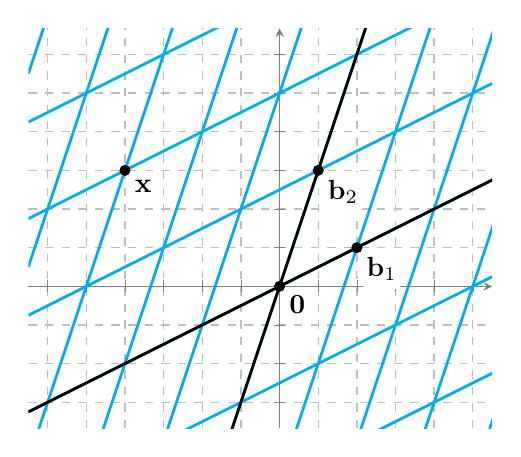
\begin{tikzpicture}[scale=1]
	% Set u and v
	\pgfmathsetmacro{\ux}{2}
	\pgfmathsetmacro{\uy}{1}
	\pgfmathsetmacro{\vx}{1}
	\pgfmathsetmacro{\vy}{3}
	\pgfmathsetmacro{\xcoor}{-4}
	\pgfmathsetmacro{\ycoor}{3}
	% Begin Axis
	\begin{axis}[axis x line=center, axis y line=middle,
	xmin=-6.5, xmax=5.5,
	ymin=-3.5, ymax=6.5,
	xtick={-6,...,5}, ytick={-3,...,7},
	xticklabels={,,}, yticklabels={,,},
	scale only axis, axis equal, height=2in,
	gray,
	grid=major, grid style={line width=.5pt, draw=gray!50, dashed}]
	% Plot alternate coordinate system
	\foreach \yi in {-10,...,10}{
		\addplot[-, cyan, line width=1pt, domain=-6.5:6.5] {(\uy/\ux)*(x-\yi*\vx)+\vy*\yi};
	}
	\foreach \xi in {-10,...,10}{
		\addplot[-, cyan, line width=1pt, domain=-6.5:6.5] {(\vy/\vx)*(x-\xi*\ux)+\uy*\xi};
	}
	\addplot[-, black, line width=1pt, domain=-6.5:6.5] {(\uy/\ux)*x};
	\addplot[-, black, line width=1pt, domain=-6.5:6.5] {(\vy/\vx)*x};
	% Plot vectors
	\fill[black] (0,0) circle (2pt) node[below right, fill=white, rounded corners=0.2cm] {$\vect{0}$};
	\fill[black] (\ux,\uy) circle (2pt) node[below right, fill=white, rounded corners=0.2cm] {$\vect{b}_1$};
	\fill[black] (\vx,\vy) circle (2pt) node[below right, fill=white, rounded corners=0.2cm] {$\vect{b}_2$};
	\fill[black] (\xcoor,\ycoor) circle (2pt) node[below right, fill=white, rounded corners=0.2cm] {$\vect{x}$};
	\end{axis}
	\end{tikzpicture}
	\end{center}
	\end{multicols}
\end{exercise}

\vfill

\begin{boxthm}
	\textbf{Theorem} \\
	If a vector space $H$ has a basis of $n$ vectors, then every basis for $H$ must consist of exactly $n$ vectors.
\end{boxthm}
\vspace{-1em}
\begin{boxdef}
	The \textbf{dimension} of a vector space $H$, denoted $\dim H$, is the number of vectors in a basis for $H$.
\end{boxdef}

\begin{boxme}
	The dimension of $\Nul A$ is the number of free variables in the equation $\Axz$. \\
	The dimension of $\Col A$ is the number of pivot columns in $A$.
\end{boxme}


\newpage

\begin{boxdef}
	The \textbf{rank} of $A$ is the dimension of the column space of $A$.
\end{boxdef}

\begin{boxthm}
	\textbf{Theorem 2.14.}
	\textbf{The Rank Theorem} \\
	The dimension of the column space and the row space of an $m\times n$ matrix $A$ are equal. This common dimension, the rank of $A$, also equals the number of pivot positions in $A$ and satisfies the equation
	\vspace{-1em}
	$$ \rank A + \dim\Nul A = n. $$
\end{boxthm}


\begin{exercise} % 4.5.13 & 15
	Determine the dimensions of the null space and column space for $A$.
	\begin{multicols}{2}
	\begin{enumerate}[(a)]
		\item $$A=\begin{bmatrix}1&-5&-5&3&-6\\0&1&7&-2&2\\0&0&0&-6&-9\\0&0&0&0&1\end{bmatrix}$$
		\vfill
		
		$\boldsymbol{\dim\Nul A=}$ \\[1em]
		$\boldsymbol{\rank A = \dim\Col A=}$

	\end{enumerate}
	\end{multicols}
\end{exercise}
\vfill


\begin{boxthm}
	\textbf{Theorem} \\
	If a subspace $H$ of $\mathbb{R}^n$ has a basis $\B=\vectset[b]{1}{p}$, then any set in $H$ containing more than $p$ vectors must be linearly dependent.
\end{boxthm}
\vspace{-1em}
\begin{boxthm}
	\textbf{Theorem 2.15.}
	\textbf{The Basis Theorem} \\
	Let $H$ be a $p$-dimensional subspace of $\mathbb{R}^n$. Any linearly independent set of vectors of exactly $p$ elements in $H$ is automatically a basis for $H$. Any set of exactly $p$ elements that spans $H$ is automatically a basis for $H$.
\end{boxthm}


\begin{exercise} % 4.5.Custom
	Use the above theorems to answer the questions here.
	\begin{multicols}{2}
		\begin{enumerate}[(a)]
			\item The set of vectors below span $\R^5$.
			$$\left\{
			\begin{bmatrix}1\\2\\1\\0\\1\end{bmatrix},
			\begin{bmatrix}1\\0\\1\\1\\1\end{bmatrix},
			\begin{bmatrix}1\\2\\1\\3\\1\end{bmatrix},
			\begin{bmatrix}1\\2\\3\\1\\1\end{bmatrix},
			\begin{bmatrix}1\\0\\0\\0\\0\end{bmatrix},
			\begin{bmatrix}0\\0\\0\\0\\1\end{bmatrix}
			\right\}$$
			Is this set a basis for $\R^5$? Explain.
			
			\columnbreak
			\item 
			$$\left\{
			\begin{bmatrix}1\\0\\0\end{bmatrix},
			\begin{bmatrix}1\\4\\0\end{bmatrix},
			\begin{bmatrix}1\\2\\1\end{bmatrix}
			\right\}$$
			Is this set a basis for $\R^3$? Explain.
		\end{enumerate}
	\end{multicols}
\end{exercise}
\vfill

\newpage


% CH 3
\chapter{Matrix Operations}
\chaptermark{Determinants}

% SEC 3.1
\section{Introduction to Determinants}
\name

\begin{boxme}
	Given a matrix $A$, we define a submatrix, $A_{ij}$, by deleting the $i$th row and $j$th column. \par
	
	\textbf{Example:} Given $A$ below, you get $A_{23}$ by deleting the 2nd row and 3rd column from $A$.
	\begin{align*}
	A = 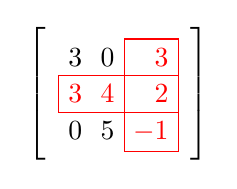
\begin{tikzpicture}[baseline=-0.5ex]%\usetikzlibrary{arrows,matrix,positioning}
	\matrix[matrix of math nodes, matrix anchor=east,
	left delimiter={[},right delimiter={]},
	every odd column/.style={anchor=base east},
	every even column/.style={anchor=base east},
	column 3/.style={color=red},
	row 2/.style={color=red},
	ampersand replacement=\&
	] (A) at (0,0)
	{
		3 \& 0 \&  3  \\
		3 \& 4 \&  2  \\
		0 \& 5 \& -1  \\
	};
	\draw[color=red] (A-2-1.north west) rectangle (A-2-3.south east);
	\draw[color=red] (A-1-2.north east) rectangle (A-3-3.south east);
	\end{tikzpicture}
	\quad
	&\xrightarrow[\text{\& 3rd Column}]{\text{Delete 2nd Row}}
	\quad
	A_{23} = \begin{bmatrix} 3&0 \\ 0&5 \end{bmatrix}
	\end{align*}
\end{boxme}

\begin{exercise} % 3.1.5
	Given $A=\begin{bmatrix}6&7&-5\\2&0&4\\5&2&3\end{bmatrix}$, determine the following.
	\begin{multicols}{3}
		\begin{enumerate}[(a)]
			\item $\det A_{11}$
			\item $\det A_{12}$
			\item $\det A_{13}$
		\end{enumerate}
	\end{multicols}
\end{exercise}
\vfill

\begin{boxme}
	\vspace{-1em}
	\begin{multicols}{2}
		The $(i,j)$-cofactor of $A$ is defined as.
		\begin{align*}
		C_{ij} &= (-1)^{i+j}\det A_{ij}
		\end{align*}
		\textbf{Example:} (uses $A_{23}$ from previous example)
		\begin{align*}
		C_{23} &= (-1)^{2+3}\det A_{23} \\
		&= (-1)^5\begin{vmatrix} 3&0 \\ 0&5 \end{vmatrix} \\
		&= (-1)(3\cdot 5 - 0) = -15
		\end{align*}
		
		\columnbreak
		
		The factor $(-1)^{i+j}$ determines the following pattern of signs:
		$$\begin{bmatrix}[c] +&-&+&\cdots \\ -&+&-& \\ +&-&+& \\ \vdots&&&\ddots \end{bmatrix}$$
	\end{multicols}
\end{boxme}
\begin{boxdef}
	For $n\geq 2$, the \textbf{determinant} of an $n\times n$ matrix $A=[a_{ij}]$ is the sum of $n$ terms of the form $\pm a_{1j}\det A_{1j}$, with plus and minus signs alternating, where the entries $a_{11},a_{12},\ldots,a_{1n}$ are from the first row of $A$. 
	\begin{align*}
	\det A &= a_{11}\det A_{11} - a_{12}\det A_{12} + \cdots + (-1)^{1+n}a_{1n}\det A_{1n} \\
	&= \sum_{j=1}^n(-1)^{1+j}a_{1j}\det A_{1j}
	\end{align*}
\end{boxdef}
\begin{exercise} % 3.1.5
	Using Exercise 1 and the above definition, compute the determinant of $A=\begin{bmatrix}6&7&-5\\2&0&4\\5&2&3\end{bmatrix}$.
	\vspace{-1ex}
	\begin{align*}
	\det A &= a_{11}\det A_{11} - a_{12}\det A_{12} + \cdots + (-1)^{1+n}a_{1n}\det A_{1n} \\
	&= (6)\det A_{11} - (7)\det A_{12} + (-5)\det A_{13} \\[1em]
	&=
	\end{align*}
\end{exercise}
\vfill


\newpage

\begin{boxthm}
	\textbf{Theorem 3.1.} \\
	The determinant of a $n\times n$ matrix $A$ can be computed by a cofactor expansion across any row or down any column. The expansion across the $i$th row using the cofactors $C_{ij} = (-1)^{i+j}\det A_{ij}$ is
	$$ \det A = a_{i1}C_{i1} + a_{i2}C_{i2} + \cdots + a_{in}C_{in}. $$
	The cofactor expansion down the $j$th column is
	$$ \det A = a_{1j}C_{1j} + a_{2j}C_{2j} + \cdots + a_{nj}C_{nj}. $$
\end{boxthm}

\begin{exercise} % 3.1.9
	Compute the determinant by cofactor expansion. At each step, try to choose a row or column that involves the least amount of computation. \\
	
	$\begin{vmatrix}1&6&3&9\\0&7&0&3\\0&2&0&1\\4&-7&0&7\end{vmatrix}$
\end{exercise}
\vfill


\begin{boxthm}
	\textbf{Theorem 3.2.} \\
	If $A$ is a triangular matrix, then $\det A$ is the product of the entries on the main diagonal of $A$.
\end{boxthm}
\begin{exercise} % 3.1.
	Compute the following determinants.
	\begin{multicols}{3}
%		\pgfmathsetseed{101}
%	\begin{enumerate}[(a)]
%		\item 	$\begin{vmatrix}
%				\Rand&\Rand&\Rand\\
%				0&\Rand&\Rand\\
%				0&0&\Rand
%				\end{vmatrix}$
%		\item 	$\begin{vmatrix}
%				\Rand&-\Rand&\Rand&\Rand\\
%				0&-\Rand&\Rand&-\Rand\\
%				0&0&\Rand&\Rand\\
%				0&0&0&-\Rand
%				\end{vmatrix}$
%		\item	$\begin{vmatrix}
%				\Rand&\Rand&\Rand&\Rand&\Rand&\Rand\\
%				0&\Rand&\Rand&\Rand&\Rand&\Rand\\
%				0&0&\Rand&\Rand&\Rand&\Rand\\
%				0&0&0&\Rand&\Rand&\Rand\\
%				0&0&0&0&\Rand&\Rand\\
%				0&0&0&0&0&0
%				\end{vmatrix}$
%	\end{enumerate}
	\begin{enumerate}[(a)]
		\item
			$\begin{vmatrix}
			5&1&3\\
			0&3&3\\
			0&0&2
			\end{vmatrix}$
		\item 
			$\begin{vmatrix}
			3&-1&7& 5\\
			0&-3&2&-1\\
			0& 0&4& 7\\
			0& 0&0&-2
			\end{vmatrix}$
		\item
			$\begin{vmatrix}
			4&7&4&6&1&6\\
			0&1&6&4&4&1\\
			0&0&5&3&1&4\\
			0&0&0&1&4&1\\
			0&0&0&0&4&5\\
			0&0&0&0&0&0
			\end{vmatrix}$
	\end{enumerate}
	\end{multicols}
\end{exercise}
\vspace{1in}

\newpage

\section{Properties of Determinants}
\name

Read the Properties of Determinants Section outline from a different book and answer the following questions.  This reading assignment is due Wednesday, February 26, 2020 at the beginning of class.
\begin{boxthm}
	\textbf{Theorem 3.3.} \\
	Let $A$ be a square matrix.
	\begin{enumerate}[(a)]
		\item If a multiple of one row of $A$ is added to another row to produce $B$, then $\det B = \det A$.
		\item If two rows of $A$ are interchanged to produce $B$, then $\det B = -\det A$.
		\item If one row of $A$ is multiplied by $k$ to produce $B$, then $\det B = k\det A$.
	\end{enumerate}
\end{boxthm}

\begin{exercise} % 3.2.9
	Find the determinant of $A=\begin{bmatrix}1&-1&-3&0\\0&1&5&4\\-1&0&5&3\\3&-3&-2&3\end{bmatrix}$ by row reducing to a matrix of row echelon form.
\end{exercise}
\vfill

\begin{boxthm}
	\textbf{Theorem 3.4.} \\
	Let $A$ be a square matrix. $A$ is invertible if and only if $\det A \ne 0$.
\end{boxthm}

\begin{exercise}
Does the matrix, $A$, from the previous exercise have an inverse? Why or why not?
\end{exercise}

\vspace{2cm}

\newpage

\begin{boxthm}
	\textbf{Theorem 3.5.} \\
	If $A$ is a square matrix, then $\det A = \det A^T$.
\end{boxthm}

\begin{boxthm}
	\textbf{Theorem 3.6.} \\
	If $A$ and $B$ are both $n \times n$ matrices, then $\det AB = \det A \det B$.
\end{boxthm}

\begin{exercise}
Suppose $A$ and $B$ are both $3 \times 3$ matrices where $\det A = 2$ and $\det B = -3$. Use the theorems from both sides to determine each of the following:

\begin{enumerate}[(a)]

\item $\det AB$

\vfill

\item $\det A^T$

\vfill

\item $\det 5A$

\vfill

\item $\det B^{-1}$

\vfill

\item $\det A^3$

\vfill

\end{enumerate}

\end{exercise}

\newpage

\section{Cramer's Rule and Volume}
\name

\begin{boxthm}
	\textbf{Theorem 3.7: Cramer's Rule.} \\
	Let $A$ be an $n \times n$ invertible matrix. For any $\vect{b} \in \mathbb{R}^n$, the unique solution $\vect{x}$ of $A\vect{x}=\vect{b}$ has entries given by $$x_i = \frac{\det A_i(\vect{b})}{\det A}, \hspace{1cm} i = 1,2,...,n.$$
\end{boxthm}

\begin{exercise}
Consider the following system:

\[\systeme[x_1,x_2]{
	 5x_1	+	7x_2	= 3,
	2x_1	+	4x_2	= 1
	}
\]

\begin{enumerate}[(a)]

\item Rewrite the system in the form $A\vect{x}=\vect{b}$.
\vfill

\item Verify that $\det A \ne 0$, so that Cramer's Rule will apply.
\vfill

\item Solve the system using Cramer's Rule.
\vfill
\vfill
\vfill

\end{enumerate}
\end{exercise}

\newpage

\begin{boxthm}
	\textbf{Theorem 3.9.} \\
	If $A$ is a $2 \times 2$ matrix, the area of the parallelogram determined by by the columns of $A$ is $|\det A|$. If $A$ is a $3 \times 3$ matrix, the volume of the parallelepiped determined by the columns of $A$ is $|\det A|$.
\end{boxthm}

\begin{boxthm}
	\textbf{Theorem 3.10.} \\
	Let $T: \mathbb{R}^2 \rightarrow \mathbb{R}^2$ be a linear transformation determined by $2 \times 2$ matrix $A$. If $S$ is a parallelogram in $\mathbb{R}^2$, then $$\{ \text{area of } T(S)\} = |\det A| \cdot \{ \text{area of } S \}.$$
	
	Alternatively, let $T: \mathbb{R}^3 \rightarrow \mathbb{R}^3$ be a linear transformation determined by $3 \times 3$ matrix $A$. If $S$ is a parallelepiped in $\mathbb{R}^3$, then $$\{ \text{volume of } T(S)\} = |\det A| \cdot \{ \text{volume of } S \}.$$
\end{boxthm}

\begin{exercise}

Let $S$ be the parallelogram determined by the vectors $\vect{b_1} = \begin{bmatrix}2\\1\end{bmatrix}$ and $\vect{b_2} = \begin{bmatrix}1\\3\end{bmatrix}$.

\begin{enumerate}[(a)]

\item Shade in $S$ in the picture below. Then, use a determinant to find the area of $S$.

\hfill 	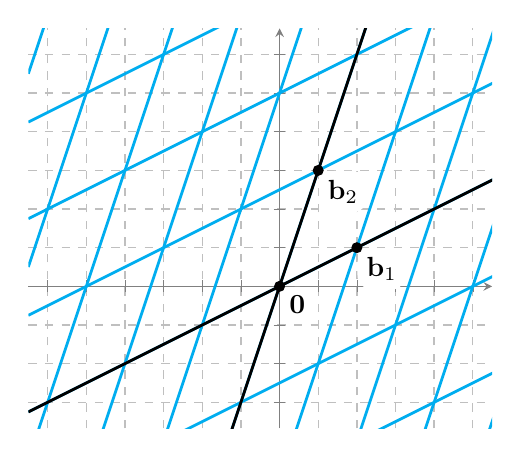
\begin{tikzpicture}[scale=1]
	% Set u and v
	\pgfmathsetmacro{\ux}{2}
	\pgfmathsetmacro{\uy}{1}
	\pgfmathsetmacro{\vx}{1}
	\pgfmathsetmacro{\vy}{3}
	\pgfmathsetmacro{\xcoor}{-4}
	\pgfmathsetmacro{\ycoor}{3}
	% Begin Axis
	\begin{axis}[axis x line=center, axis y line=middle,
	xmin=-6.5, xmax=5.5,
	ymin=-3.5, ymax=6.5,
	xtick={-6,...,5}, ytick={-3,...,7},
	xticklabels={,,}, yticklabels={,,},
	scale only axis, axis equal, height=2in,
	gray,
	grid=major, grid style={line width=.5pt, draw=gray!50, dashed}]
	% Plot alternate coordinate system
	\foreach \yi in {-10,...,10}{
		\addplot[-, cyan, line width=1pt, domain=-6.5:6.5] {(\uy/\ux)*(x-\yi*\vx)+\vy*\yi};
	}
	\foreach \xi in {-10,...,10}{
		\addplot[-, cyan, line width=1pt, domain=-6.5:6.5] {(\vy/\vx)*(x-\xi*\ux)+\uy*\xi};
	}
	\addplot[-, black, line width=1pt, domain=-6.5:6.5] {(\uy/\ux)*x};
	\addplot[-, black, line width=1pt, domain=-6.5:6.5] {(\vy/\vx)*x};
	% Plot vectors
	\fill[black] (0,0) circle (2pt) node[below right, fill=white, rounded corners=0.2cm] {$\vect{0}$};
	\fill[black] (\ux,\uy) circle (2pt) node[below right, fill=white, rounded corners=0.2cm] {$\vect{b}_1$};
	\fill[black] (\vx,\vy) circle (2pt) node[below right, fill=white, rounded corners=0.2cm] {$\vect{b}_2$};
	%\fill[black] (\xcoor,\ycoor) circle (2pt) node[below right, fill=white, rounded corners=0.2cm] {$\vect{x}$};
	\end{axis}
	\end{tikzpicture}

\item Find the area of the image of $S$ under the mapping $\vect{x} \rightarrow A\vect{x}$ where $A =\begin{bmatrix}5&-1\\2&5\end{bmatrix}$.
\vfill
\vfill

\end{enumerate}

\end{exercise}

% MISSING SECTIONS 3.2-3.3, 4.1-4.2
% Missed a few sections when Romy was born. (3.2, 3.3, 4.1, 4.2)
% SEC 3.3
%\section{Cramer's Rule, Volume, and Linear Transformations}


\newpage



% CH 4
\chapter{Vector Spaces}
\chaptermark{Vector Spaces}

%% Missed a few sections when Romy was born. (4.1, 4.2)
%% SEC 4.1
%%\section{Vector Spaces and Subspaces}
%% SEC 4.2
%%\section{Null Spaces, Column Spaces, and Linear Transformations}


% SEC 4.3
\setcounter{section}{2}
\section{Linearly Independent Sets; Bases}
\name[2in]


\begin{boxdef}
An indexed set of vectors $\B=\vectset[b]{1}{p}$ in $V$ is a \textbf{basis} for a subspace $H$ of $V$ if
\begin{enumerate}[(i)]
	\item $\B$ is a linearly independent set, and
	\item $H=\Span\vectset[b]{1}{p}$, i.e., the vectors $\vect{b}_1,\ldots,\vect{b}_p$ span $H$ (and no more than $H$).
\end{enumerate}
\end{boxdef}


\begin{exercise} % 4.3.1
	Determine if the set is linearly independent, if it spans $\R^3$, and if it is a basis for $\R^3$. Show work or explain your answer.
	$$ \left\{
	\begin{bmatrix}2\\2\\0\end{bmatrix},
	\begin{bmatrix}0\\2\\2\end{bmatrix},
	\begin{bmatrix}0\\2\\0\end{bmatrix}
	\right\} $$
	Circle all that apply:
	\begin{center}
	\shortstack{\textbf{Linearly Independent?} \\[1ex]
		\textbf{Yes \qquad No}} \hspace{5em}
	\shortstack{\textbf{\textbf{Spans} $\boldsymbol{\R^3}$?} \\[1ex]
		\textbf{Yes \qquad No}} \hspace{5em}
	\shortstack{\textbf{\textbf{Is a Basis for} $\boldsymbol{\R^3}$?} \\[1ex]
		\textbf{Yes \qquad No}}
	\end{center}
\end{exercise}
\vfill


\begin{exercise} % 4.3.5
	Determine if the set is linearly independent, if it spans $\R^3$, and if it is a basis for $\R^3$. Show work or explain your answer.
	$$ \left\{
	\begin{bmatrix}1\\-3\\0\end{bmatrix},
	\begin{bmatrix}-2\\3\\0\end{bmatrix},
	\begin{bmatrix}0\\0\\0\end{bmatrix},
	\begin{bmatrix}0\\-3\\5\end{bmatrix}
	\right\} $$
	Circle all that apply:
	\begin{center}
		\shortstack{\textbf{Linearly Independent?} \\[1ex]
			\textbf{Yes \qquad No}} \hspace{5em}
		\shortstack{\textbf{\textbf{Spans} $\boldsymbol{\R^3}$?} \\[1ex]
			\textbf{Yes \qquad No}} \hspace{5em}
		\shortstack{\textbf{\textbf{Is a Basis for} $\boldsymbol{\R^3}$?} \\[1ex]
			\textbf{Yes \qquad No}}
	\end{center}
\end{exercise}
\vfill


\newpage

\begin{boxme}
	To find a basis for $\Nul A$, write the general solution of $\Axz$ in parametric vector form. The vectors in the solution form a basis for $\Nul A$ (whenever $\Nul A \neq \{\vect{0}\}$)
\end{boxme}
\begin{boxthm}
	\textbf{Theorem 4.6.} \\
	The pivot columns of a matrix $A$ form a basis for $\Col A$.
\end{boxthm}

\begin{exercise} % 4.3.13
	Assume that $A$ is row equivalent to $B$.
	\begin{align*}
	A &= \begin{bmatrix} -2&4&-2&-4 \\ 2&-6&-6&1 \\ -3&8&5&-3 \end{bmatrix} &
	B &= \begin{bmatrix} 1&0&9&5 \\ 0&2&8&3 \\ 0&0&0&0 \end{bmatrix}
	\end{align*}
	\begin{multicols}{2}
		\begin{enumerate}[(a)]
			\item Find a basis for $\Nul A$.
			\item Find a basis for $\Col A$.
		\end{enumerate}
	\end{multicols}
\end{exercise}
\vfill


\begin{boxthm}
	\textbf{Theorem 4.5.}
	\textbf{The Spanning Set Theorem} \\
	Let $S=\vectsetvp$ be a set in $V$, and let $H=\Span\vectsetvp$.
	\begin{enumerate}[a.]
		\item If one of the vectors in $S$---say, $\vect{v}_k$---is a linear combination of the remaining vectors in $S$, then the set formed from $S$ by removing $\vect{v}_k$ still spans $H$.
		\item If $H\neq\{\vect{0}\}$, some subset of $S$ is a basis for $H$.
	\end{enumerate}
\end{boxthm}
\begin{exercise} % 4.3.19
	Let $\vect{v}_1 = \begin{bmatrix} 1\\2\\3 \end{bmatrix}$, $\vect{v}_2 = \begin{bmatrix} 3\\2\\1 \end{bmatrix}$, and $\vect{v}_3 = \begin{bmatrix} 4\\4\\4 \end{bmatrix}$. Note that $\vect{v}_1+\vect{v}_2=\vect{v}_3$. Find a basis for the subspace $H=\Span\{\vect{v}_1,\vect{v}_2,\vect{v}_3\}$.
\end{exercise}
\vspace{1in}


\newpage


% SEC 4.4
\section{Coordinate Systems}
\name

\begin{boxdef}
	Suppose $\B=\vectset[b]{1}{n}$ is a basis for $V$ and $\vect{x}$ is in $V$. The \textbf{coordinates of $\boldsymbol{\vect{x}}$ relative to the basis $\boldsymbol{\B}$} (or the $\boldsymbol{\B}$\textbf{-coordinates of} $\boldsymbol{\vect{x}}$) are the weights $c_1,\ldots,c_n$ such that $\vect{x} = c_1\vect{b}_1 + \cdots + c_n\vect{b}_n$.
	\begin{align*}
	\vectB &= \begin{bmatrix}[c]c_1 \\ \vdots \\ c_n\end{bmatrix}
	\end{align*}
	We call $\vectB$ the \textbf{coordinate vector of $\boldsymbol{\vect{x}}$ (relative to $\boldsymbol{\B}$)} or the \textbf{$\boldsymbol{\B}$-coordinate vector of $\boldsymbol{\vect{x}}$}.
\end{boxdef}


\begin{exercise} % 4.4.Custom (Graphical Interpretation)
	\begin{multicols}{2}
	The vectors $\vect{b}_1=\begin{bmatrix}2\\1\end{bmatrix}$, $\vect{b}_2=\begin{bmatrix}1\\3\end{bmatrix}$, and $\vect{x}=\begin{bmatrix}-4\\3\end{bmatrix}$ are shown in the figure. The vectors $\vect{b}_1$ and $\vect{b}_2$ provide a basis for $\R^2$, $\B=\{\vect{b}_1,\vect{b}_2\}$. This basis provides a new ``coordinate system'' as shown in the figure.
	
	Using the figure, find $\vectB = \begin{bmatrix}c_1 \\ c_2\end{bmatrix}$.
	
	\columnbreak
	
	\begin{center}
	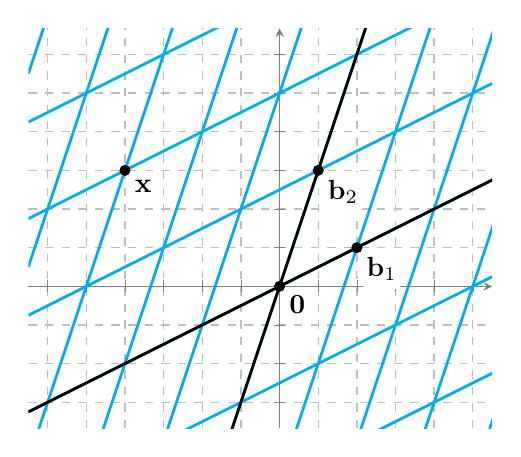
\begin{tikzpicture}[scale=1]
	% Set u and v
	\pgfmathsetmacro{\ux}{2}
	\pgfmathsetmacro{\uy}{1}
	\pgfmathsetmacro{\vx}{1}
	\pgfmathsetmacro{\vy}{3}
	\pgfmathsetmacro{\xcoor}{-4}
	\pgfmathsetmacro{\ycoor}{3}
	% Begin Axis
	\begin{axis}[axis x line=center, axis y line=middle,
	xmin=-6.5, xmax=5.5,
	ymin=-3.5, ymax=6.5,
	xtick={-6,...,5}, ytick={-3,...,7},
	xticklabels={,,}, yticklabels={,,},
	scale only axis, axis equal, height=2in,
	gray,
	grid=major, grid style={line width=.5pt, draw=gray!50, dashed}]
	% Plot alternate coordinate system
	\foreach \yi in {-10,...,10}{
		\addplot[-, cyan, line width=1pt, domain=-6.5:6.5] {(\uy/\ux)*(x-\yi*\vx)+\vy*\yi};
	}
	\foreach \xi in {-10,...,10}{
		\addplot[-, cyan, line width=1pt, domain=-6.5:6.5] {(\vy/\vx)*(x-\xi*\ux)+\uy*\xi};
	}
	\addplot[-, black, line width=1pt, domain=-6.5:6.5] {(\uy/\ux)*x};
	\addplot[-, black, line width=1pt, domain=-6.5:6.5] {(\vy/\vx)*x};
	% Plot vectors
	\fill[black] (0,0) circle (2pt) node[below right, fill=white, rounded corners=0.2cm] {$\vect{0}$};
	\fill[black] (\ux,\uy) circle (2pt) node[below right, fill=white, rounded corners=0.2cm] {$\vect{b}_1$};
	\fill[black] (\vx,\vy) circle (2pt) node[below right, fill=white, rounded corners=0.2cm] {$\vect{b}_2$};
	\fill[black] (\xcoor,\ycoor) circle (2pt) node[below right, fill=white, rounded corners=0.2cm] {$\vect{x}$};
	\end{axis}
	\end{tikzpicture}
	\end{center}
	\end{multicols}
\end{exercise}
\vspace{1in}


\begin{boxdef}
	For coordinates in $\R^n$, the \textbf{change-of-coordinates matrix} from $\B$ to the standard basis in $\R^n$, $$P_\B=\begin{bmatrix}\vect{b}_1&\cdots&\vect{b}_n\end{bmatrix},$$
	is used to transform $\vectB$ into $\vect{x}$ via the \textbf{change-of-coordinates equation}, $\vect{x}=P_\B\vectB$.
\end{boxdef}
\begin{exercise} % 4.4.7&9 Sort of
	Given $\B=\left\{ \begin{bmatrix}1\\-1\\-2\end{bmatrix}, \begin{bmatrix}-2\\3\\4\end{bmatrix}, \begin{bmatrix}1\\-1\\4\end{bmatrix} \right\}$ and $\vectB=\begin{bmatrix}-1\\1\\-3\end{bmatrix}$, answer the following.
	\begin{multicols}{2}
		\begin{enumerate}[(a)]
			\item Find the change-of-coordinates matrix, $P_\B$.
			\item Use $P_\B$ to find $\vect{x}$.
		\end{enumerate}
	\end{multicols}
\end{exercise}
\vfill


\newpage


\begin{boxdef}
	The \textbf{change-of-coordinates equation} is $\vect{x}=P_\B\vectB$. To find $\vectB$, you may solve the linear system $P_\B\vectB=\vect{x}$ or use the equation $\vectB=P_\B^{-1}\vect{x}$.
\end{boxdef}
\begin{exercise} % 4.4.5
	Find the coordinate vector $\vectB$ of $\vect{x}$ relative to the basis $\B=\{\vect{b}_1,\vect{b}_2\}$.
	\begin{align*}
	\vect{b}_1 &= \begin{bmatrix}2\\3\end{bmatrix} &
	\vect{b}_2 &= \begin{bmatrix}-5\\-1\end{bmatrix} &
	\vect{x} &= \begin{bmatrix}3\\-2\end{bmatrix}
	%& \vectB &=\begin{bmatrix}-1\\-1\end{bmatrix}
	\end{align*}
%% \R^3 Version might be too long:
%	Find the coordinate vector $\vectB$ of $\vect{x}$ relative to the basis $\B=\{\vect{b}_1,\vect{b}_2,\vect{b}_3\}$.
%	\begin{align*}
%	\vect{b}_1 &= \begin{bmatrix}1\\-1\\-3\end{bmatrix} &
%	\vect{b}_2 &= \begin{bmatrix}4\\-3\\-12\end{bmatrix} &
%	\vect{b}_3 &= \begin{bmatrix}2\\-2\\10\end{bmatrix} &
%	\vect{x} &= \begin{bmatrix}-5\\4\\-1\end{bmatrix}
%	%& \vectB &=\begin{bmatrix}1\\-1\\-1\end{bmatrix}
%	\end{align*}
\end{exercise}
\vfill


\begin{boxthm}
	\textbf{Theorem 4.8.} \\
	Let $\B=\vectset[b]{1}{n}$ be a basis for a vector space $V$. Then the coordinate mapping $\vect{x}\mapsto\vectB$ is a one-to-one linear transformation from $V$ onto $\R^n$.
\end{boxthm}
\vspace{-1em}
\begin{boxme}
	If a vector space $V$ has a basis of $n$ vectors, Theorem 4.8 says that vectors from $V$ will ``act like'' vectors in $\R^n$ under linear transformations. This is particularly useful for vector spaces whose standard basis is something other than the usual coordinate vectors we're used to. For example, the standard basis for, $\Poly_n$, the vector space of polynomials of degree at most $n$, is $\B=\{1,t,t^2,...,t^n\}$. Theorem 4.8 allows us to rewrite polynomials in $\Poly_n$ using coordinates in $\R^{n+1}$ instead (since $\B$ contains $n+1$ vectors).
\end{boxme}
\begin{exercise} % 4.4.13
	The set $\B=\{ 1-t^2, -2t+t^2, 1+t-t^2 \}$ is a basis for $\Poly_2$. Find $\vectB[p]$, the coordinate vector of $\vect{p}(t)=1-7t+2t^2$ relative to $\B$. \\

	Hint: You are trying to find $c_1$, $c_2$, and $c_3$, so that
	\begin{align*}
	c_1(1-t^2)+c_2(-2t+t^2)+c_3(1+t-t^2) &= 1-7t+2t^2. \\
	\text{Reordering terms gives:}\quad
	(c_1+c_3) + (-2c_2+c_3)t + (-c_1+c_2-c_3)t^2 &= 1-7t+2t^2.
	\end{align*}
	Noting that the coefficients on the left and right hand side have to match, use this equation to come up with a system of 3 linear equations in the unknowns $c_1$, $c_2$, and $c_3$. Solving the system will give you $\vectB[p]$.
\end{exercise}
\vfill


\newpage


% SEC 4.5
\section{The Dimension of a Vector Space}
\name[2in]


\begin{boxthm}
	\textbf{Theorem 4.10.} \\
	If a vector space $V$ has a basis of $n$ vectors, then very basis for $V$ must consist of exactly $n$ vectors.
\end{boxthm}
\vspace{-1em}
\begin{boxdef}
	The \textbf{dimension} of a vector space $V$, denoted $\dim V$, is the number of vectors in a basis for $V$.
\end{boxdef}

\begin{exercise} % 4.5.1 Custom
	$$\left\{ \begin{bmatrix}[c] 4s - 2t \\ -3s + t \\ 3t \end{bmatrix} : s,t \text{ in } \R \right\}$$
	\begin{enumerate}[(a)]
		\item Find a basis for the subspace given above. \\
		(Hint: First write the subspace as a linear combination of vectors with $s$ and $t$ as parameters.)
		\vfill
		\item State the dimension of the subspace.
		\vspace{2em}
	\end{enumerate}
\end{exercise}


\begin{boxme}
	The dimension of $\Nul A$ is the number of free variables in the equation $\Axz$. \\
	The dimension of $\Col A$ is the number of pivot columns in $A$.
\end{boxme}


\begin{exercise} % 4.5.13 & 15
	Determine the dimensions of the null space and column space for each matrix below.
	\begin{multicols}{2}
	\begin{enumerate}[(a)]
		\item $$A=\begin{bmatrix}1&-5&-5&3&-6\\0&1&7&-2&2\\0&0&0&-6&-9\\0&0&0&0&1\end{bmatrix}$$
		\vspace{2em}
		
		$\boldsymbol{\dim\Nul A=}$ \\[1em]
		$\boldsymbol{\dim\Col A=}$
		
		\columnbreak
		
		\item $$B=\begin{bmatrix}1&0&2&6&5&-3\\0&0&1&-2&4&6\end{bmatrix}$$
		\vspace{2em}
		
		$\boldsymbol{\dim\Nul B=}$ \\[1em]
		$\boldsymbol{\dim\Col B=}$
	\end{enumerate}
	\end{multicols}
\end{exercise}
\vspace{1in}


\newpage


%\begin{exercise} % 4.5.11
%	Find the dimension of the subspace spanned by the given vectors.
%	$$ \begin{bmatrix}1\\0\\-4\end{bmatrix}, 
%	\begin{bmatrix}1\\1\\-3\end{bmatrix}, 
%	\begin{bmatrix}1\\4\\0\end{bmatrix}, 
%	\begin{bmatrix}-1\\-3\\1\end{bmatrix}$$
%\end{exercise}
%\vfill

\begin{boxthm}
	\textbf{Theorem 4.9.} \\
	If a vector space $V$ has a basis $\B=\vectset[b]{1}{n}$, then any set in $V$ containing more than $n$ vectors must be linearly dependent.
\end{boxthm}
\vspace{-1em}
\begin{boxthm}
	\textbf{Theorem 4.12.}
	\textbf{The Basis Theorem} \\
	Let $V$ be a $p$-dimensional vector space, $p\geq 1$. Any linearly independent set of vectors of exactly $p$ elements in $V$ is automatically a basis for $V$. Any set of exactly $p$ elements that spans $V$ is automatically a basis for $V$.
\end{boxthm}


\begin{exercise} % 4.5.Custom
	Use the above theorems to answer the questions here.
	\begin{multicols}{2}
		\begin{enumerate}[(a)]
			\item The set of vectors below span $\R^5$.
			$$\left\{
			\begin{bmatrix}1\\2\\1\\0\\1\end{bmatrix},
			\begin{bmatrix}1\\0\\1\\1\\1\end{bmatrix},
			\begin{bmatrix}1\\2\\1\\3\\1\end{bmatrix},
			\begin{bmatrix}1\\2\\3\\1\\1\end{bmatrix},
			\begin{bmatrix}1\\0\\0\\0\\0\end{bmatrix},
			\begin{bmatrix}0\\0\\0\\0\\1\end{bmatrix}
			\right\}$$
			Is this set a basis for $\R^5$? Explain.
			
			\columnbreak
			\item The polynomials in the set below are linearly independent.
			$$ \{1, 2t , -2+4t^2 ,  -12t+8t^3 \} $$
			Is this set a basis for $\Poly_3$? Explain
		\end{enumerate}
	\end{multicols}
\end{exercise}
\vspace{1in}


\begin{exercise} % 4.5.6
	This exercise is similar to the first one, but there is an extra step involved.
	$$\left\{ \begin{bmatrix}[c] 3a+6b-1c \\ 6a-2b-2c \\ -6a+5b+2c \\ -3a+b+c \end{bmatrix} : a,b,c \text{ in } \R \right\}$$
	\begin{enumerate}[(a)]
		\item Find a basis for the subspace given above. \\
		(Hint: Remember that basis vectors must span the space and be \emph{linearly independent}!)
		\vfill
		\item State the dimension of the subspace.
		\vspace{2em}
	\end{enumerate}
\end{exercise}


\newpage


% SEC 4.6
\section{Rank}
\name

\begin{boxdef}
	The \textbf{rank} of $A$ is the dimension of the column space of $A$.
\end{boxdef}

\begin{exercise} % 4.6.Custom
	\begin{enumerate}[(a)]
		\item Given the matrix $A$ below, determine the rank of $A$.\\
		$ A = \begin{bmatrix} 1&-3&3&-2 \\ -3&7&-1&2 \\ 0&1&-4&3 \end{bmatrix} $
		\vfill
		\item The rank of $A$ can be described in terms of the pivot positions of $A$. Write a sentence explaining this relationship.
		\vspace{.75in}
	\end{enumerate}
\end{exercise}


\begin{boxdef}
	Rows of a matrix $A$ can be viewed as vectors. If $A=\begin{bmatrix}3&0&-2\\0&4&2\end{bmatrix}$, the row vectors are $\begin{bmatrix}3\\0\\-2\end{bmatrix}$ and $\begin{bmatrix}0\\4\\2\end{bmatrix}$.
	
	The \textbf{Row Space} of $A$, denoted $\Row A$, is the set of all linear combinations of the row vectors.
\end{boxdef}
\vspace{-1em}
\begin{boxthm}
	\textbf{Theorem 4.13.} \\
	If two matrices $A$ and $B$ are row equivalent, then their row spaces are the same. If $B$ is in echelon form, the nonzero rows of $B$ form a basis for the row space of $A$ as well as for that of $B$.
\end{boxthm}

\begin{exercise} % 4.6.3 - Just row space
	The given matrices $A$ and $B$ below are row equivalent.
	\begin{align*}
	A &= \begin{bmatrix}2&-3&6&2&5\\-2&3&-3&-3&-4\\4&-6&9&5&9\\-2&3&3&-4&1\end{bmatrix} &
	B &= \begin{bmatrix}2&-3&6&2&5\\0&0&3&-1&1\\0&0&0&1&3\\0&0&0&0&0\end{bmatrix}
	\end{align*}
	\begin{enumerate}[(a)]
		\item Determine a basis for $\Row A$.
		\vfill
		\item Are the rows of $A$ linearly independent? Explain? \\
		(Hint: compare the number of rows of $A$ and $\dim\Row A$.)
		\vspace{.5in}
	\end{enumerate}
\end{exercise}


\newpage


\begin{boxthm}
	\textbf{Theorem 4.14.}
	\textbf{The Rank Theorem} \\
	The dimension of the column space and the row space of an $m\times n$ matrix $A$ are equal. This common dimension, the rank of $A$, also equals the number of pivot positions in $A$ and satisfies the equation
	\vspace{-1em}
	$$ \rank A + \dim\Nul A = n. $$
\end{boxthm}

\begin{exercise} % 4.6.8
	Suppose a $7\times 9$ matrix $A$ has 5 pivots.
	\begin{multicols}{2}
		\begin{enumerate}[(a)]
			\item What is $\rank A$? How do you know?
			\item What is $\dim\Nul A$? Explain or show work.
		\end{enumerate}
	\end{multicols}
\end{exercise}
\vspace{1.5in}


\begin{exercise} % 4.6.2
	Assume that $A$ and $B$ are row equivalent.
	\begin{align*}
	A &= \begin{bmatrix}1&-3&-2&5&-5\\2&-2&-7&13&0\\-3&9&12&-21&-9\\-2&6&0&-6&0\end{bmatrix} &
	B &= \begin{bmatrix}1&-3&-2&5&-5\\0&0&1&-1&-4\\0&0&0&0&-2\\0&0&0&0&0\end{bmatrix}
	\end{align*}
	\begin{enumerate}[(a)]
		\item Determine $\rank A$ and $\dim\Nul A$.
		\begin{align*}
		\boldsymbol{\rank A} &=		& \boldsymbol{\dim\Nul A} &=
		\end{align*}
		\item Find a basis for each of the following 3 subspaces.
			\begin{multicols}{2}
				\begin{enumerate}[(i)]
					\item $\Col A$ \vspace{1in}
					\item $\Row A$
					
					\columnbreak
					\item $\Nul A$ % BONUS problem
				\end{enumerate}
			\end{multicols}
	\end{enumerate}
	
	
% Solution:
%A basis for $\Col A$ is
%$\left\{
%\begin{bmatrix}1\\2\\-3\\-2\end{bmatrix},
%\begin{bmatrix}-2\\-7\\12\\0\end{bmatrix},
%\begin{bmatrix}-5\\0\\-9\\0\end{bmatrix}
%\right\}$.
%
%A basis for $\Row A$ is
%$\left\{
%\begin{bmatrix}1\\-3\\-2\\5\\-5\end{bmatrix},
%\begin{bmatrix}0\\0\\1\\-1\\-4\end{bmatrix},
%\begin{bmatrix}0\\0\\0\\0\\-2\end{bmatrix}
%\right\}$.
%
%A basis for $\Nul A$ is
%$\left\{
%\begin{bmatrix}3\\1\\0\\0\\0\end{bmatrix},
%\begin{bmatrix}-3\\0\\1\\1\\0\end{bmatrix}
%\right\}$.
\end{exercise}
\vspace{1in}


\newpage


% SEC 4.7
\section{Change of Basis}
\name

\begin{boxdef}
	Recall the following from section 4.4:
	
	For coordinates in $\R^n$, the \textbf{change-of-coordinates matrix} from $\B$ to the standard basis, $\E$, is the matrix $P_\B=\CoC{\B}{\E}=\begin{bmatrix}\vect{b}_1&\cdots&\vect{b}_n\end{bmatrix}.$
	$P_\B$ is used to transform $\vectB$ into $\vect{x}$ via the \textbf{change-of-coordinates equation}, $\vect{x}=P_\B\vectB$. To find $\vectB$, solve the linear system $P_\B\vectB=\vect{x}$.
\end{boxdef}

\begin{exercise} % 4.4.5 (REVIEW)
% \R^3 Version might be too long:
	Find the coordinate vector $\vectB$ of $\vect{x}$ relative to the basis $\B=\{\vect{b}_1,\vect{b}_2,\vect{b}_3\}$.
	\begin{align*}
	\vect{b}_1 &= \begin{bmatrix}1\\-1\\-3\end{bmatrix} &
	\vect{b}_2 &= \begin{bmatrix}4\\-3\\-12\end{bmatrix} &
	\vect{b}_3 &= \begin{bmatrix}2\\-2\\10\end{bmatrix} &
	\vect{x} &= \begin{bmatrix}-5\\4\\-1\end{bmatrix}
	%& \vectB &=\begin{bmatrix}1\\-1\\-1\end{bmatrix}
	\end{align*}
\end{exercise}
\vfill


\begin{boxdef}
	In 4.4, the matrix $P_\B=\CoC{\B}{\E}$ was used to translate $\B$-coordinate vectors into vectors written in the standard basis. In a similar way, we can translate between any two bases $\B$ and $\C$ using the matrix $\CoC{\B}{\C}$ described in Theorem 4.15.
\end{boxdef}
\vspace{-1em}
\begin{boxthm}
	\textbf{Theorem 4.15.} 
	(\textbf{Change-of-Coordinates Matrix from $\boldsymbol{\B}$ to $\boldsymbol{\C}$}) \\
	Let $\B=\vectset[b]{1}{n}$ and $\C=\vectset[c]{1}{n}$ be bases of a vector space $V$. Then there is a unique $n\times n$ matrix $\CoC{\B}{\C}$ such that
	$$ \vectC = \CoC{\B}{\C}\vectB. $$
	The columns of $\CoC{\B}{\C}$ are the $\C$-coordinate vectors of the vectors in the basis $\B$. That is,
	$$ \CoC{\B}{\C} = \begin{bmatrix}\vectC[b_1]&\vectC[b_2]&\cdots&\vectC[b_3]\end{bmatrix}.$$
\end{boxthm}


\begin{exercise} % 4.7.2
	Let $\B=\{\vect{b}_1,\vect{b}_2\}$ and $\C=\{\vect{c}_1,\vect{c}_2\}$ be bases for a vector space $V$, and suppose $\vect{b}_1=-\vect{c}_1+4\vect{c}_2$ and $\vect{b}_2=5\vect{c}_1-3\vect{c}_2$.
	\begin{multicols}{2}
		\begin{enumerate}[(a)]
			\item Find the change-of-coordinates matrix from $\B$ to $\C$.
			\item Find $\vectC[x]$ for $\vect{x}=5\vect{b}_1+3\vect{b}_2$.
		\end{enumerate}
	\end{multicols}
\end{exercise}
\vfill


\newpage

\begin{boxme}
	If two bases for $\R^n$ are explicitly given, $\B=\vectset[b]{1}{n}$ and $\C=\vectset[c]{1}{n}$, you may find $\CoC{\B}{\C}$ via row reduction:
	$$\begin{bmatrix}\vect{c}_1&\cdots&\vect{c}_n&\vect{b}_1&\cdots&\vect{b}_n\end{bmatrix} \xrightarrow{\text{RREF}} \begin{bmatrix}I_n&\CoC{\B}{\C}\end{bmatrix}$$
	You may also use the formula $\CoC{\B}{\C}=(P_\C)^{-1}P_\B$.
	
	If you know $\CoC{\B}{\C}$, the inverse gives you the change-of-coordinates matrix from $\C$ to $\B$: $\CoC{\C}{\B} = \left(\CoC{\B}{\C}\right)^{-1}$.
\end{boxme}


\begin{exercise} % 4.7.7
	Let $\B=\left\{ \begin{bmatrix}7\\5\end{bmatrix},\begin{bmatrix}-3\\-1\end{bmatrix} \right\}$ and $\C=\left\{ \begin{bmatrix}1\\-5\end{bmatrix},\begin{bmatrix}-2\\2\end{bmatrix} \right\}$ be two bases for $\R^2$.
	\begin{multicols}{2}
		\begin{enumerate}[(a)]
			\item Find $\CoC{\B}{\C}$.
			\item Find $\CoC{\C}{\B}$.
		\end{enumerate}
	\end{multicols}
\end{exercise}
\vfill


\begin{exercise} % 4.7.13
	In $\Poly_1$, find the change-of-coordinates matrix from the basis $\B=\{ 1-2t , 3-5t \}$ to the standard basis $\C=\{1,t\}$. Then find the $\B$-coordinate vector for $5-8t$.
	\begin{multicols}{2}
		\begin{enumerate}[(a)]
			\item Find $\CoC{\B}{\C}$.
			\item Find the $\B$-coordinate vector for $5-8t$.
		\end{enumerate}
	\end{multicols}
\end{exercise}
\vfill


%% SEC 4.9 - No In-class work
%\setcounter{section}{8}
%\section{Applications to Markov Chains}


\newpage


% CH 5
\chapter{Eigenvalues and Eigenvectors}
\chaptermark{Eigenvalues and Eigenvectors}

% SEC 5.1
\section{Eigenvectors and Eigenvalues}
\name

\begin{boxdef}
	An \textbf{eigenvector} of an $n\times n$ matrix $A$ is a nonzero vector $\vect{x}$ such that $\Axlx$ for some scalar $\lambda$. A scalar $\lambda$ is called an \textbf{eigenvector} of $A$ if there is a nontrivial solution $\vect{x}$ of $\Axlx$; such an $\vect{x}$ is called an \textbf{eigenvector corresponding to $\boldsymbol{\lambda}$}.
\end{boxdef}

\begin{exercise} % 5.1.Custom (Matrix from 5.1.15)
	Is $\vect{v}=\begin{bmatrix}1\\0\\1\end{bmatrix}$ an eigenvector of $A=\begin{bmatrix}3&3&-1\\2&8&-2\\-2&-6&4\end{bmatrix}$? If so, find the corresonding eigenvalue.
	
	Hint: Check to see if $A\vect{v}=\lambda\vect{v}$ for some $\lambda$.
\end{exercise}
\vfill


\begin{boxme}
	Given an eigenvalue $\lambda$ of a matrix $A$, an eigenvector $\vect{x}$ must be a nonzero vector satisfying $\Axlx$. In order to solve for such an $\vect{x}$, we first rewrite $\Axlx$ as follows:
	\begin{align*}
	A\vect{x} - \lambda\vect{x} &= \vect{0} \\
	A\vect{x} - \lambda I\vect{x} &= \vect{0} \\
	(A-\lambda I)\vect{x} &= \vect{0}
	\end{align*}
	If $\vect{x}$ is a nonzero solution to this homogeneous equation, $\vect{x}$ is an eigenvector of $A$ corresponding to $\lambda$.
\end{boxme}

\begin{exercise} % 5.1.12
	$$ A = \begin{bmatrix}7&4\\-3&-1\end{bmatrix}, \qquad \lambda = 1,5 $$
	\begin{multicols}{2}
		\begin{enumerate}[(a)]
			\item Compute $(A-\lambda I)$ for $\lambda=1$.
			
			$\begin{bmatrix}7&4\\-3&-1\end{bmatrix}-1\begin{bmatrix}1&0\\0&1\end{bmatrix}=$
			\vspace{2em}
			\item Find an eigenvector of $A$ with eigenvalue 1.
			\columnbreak
			\item Compute $(A-\lambda I)$ for $\lambda=5$.
			
			\phantom{$\begin{bmatrix}7&4\\-3&-1\end{bmatrix}-5\begin{bmatrix}1&0\\0&1\end{bmatrix}=$}
			\vspace{2em}
			\item Find an eigenvector of $A$ with eigenvalue 5.
		\end{enumerate}
	\end{multicols}
\end{exercise}
\vfill


\newpage


\begin{boxthm}
	\textbf{Theorem 5.1.} \\
	The eigenvalues of a triangular matrix are the entries on its main diagonal.
\end{boxthm}
\vspace{-1em}

\begin{boxme}
	Note: If 0 is an eigenvalue of $A$, then we have some eigenvector $\vect{x}$ that satisfies $A\vect{x}=0\vect{x}$. In other words, $\Axz$ has a nontrivial solution. According to the invertible matrix theorem, this happens precisely when $A$ is \textbf{not invertible}. So 0 is an eigenvalue of $A$ if, and only if, $A$ is not invertible!
\end{boxme}

\begin{exercise} % 5.1.17&19
	Use Theorem 5.1 or the note above along with the Invertible Matrix Theorem to answer the following questions.
	\begin{multicols}{2}
		\begin{enumerate}[(a)]
			\item Find the eigenvalues of the matrix.
			$$A=\begin{bmatrix}0&0&0\\0&-3&2\\0&0&7\end{bmatrix}$$
			\columnbreak 
			\item Find one eigenvalue of the matrix without calculations. Explain your answer.
			$$B=\begin{bmatrix}-1&3&7\\-1&3&7\\-1&3&7\end{bmatrix}$$
		\end{enumerate}
	\end{multicols}
\end{exercise}
\vfill


\begin{boxme}
	For an $n\times n$ matrix $A$, the set of all the eigenvectors corresponding to an eigenvalue $\lambda$ along with the zero vector forms a subspace of $\R^n$. This subspace, the set of all solutions to $(A-I\lambda)\vect{x}=\vect{0}$ (or the null space of ($A-\lambda I$)), is called the \textbf{eigenspace} of $A$ corresponding to $\lambda$.
\end{boxme}

\begin{exercise} % 5.1.13
	Find a basis for the eigenspace corresponding to the given eigenvalue.
	$$ A = \begin{bmatrix}4&0&1\\-2&1&0\\-2&0&1\end{bmatrix}, \qquad \lambda = 2 $$
	Hint: Find a basis for the null space of $(A-\lambda I)$.
\end{exercise}
\vfill

%\begin{exercise} % 5.1.10
%	Find a basis for the eigenspace corresponding to the given eigenvalue.
%	$$ A = \begin{bmatrix}10&-9\\4&-2\end{bmatrix}, \qquad \lambda = 4 $$
%	Hint: Find a basis for the null space of $(A-\lambda I)$.
%\end{exercise}
%\vfill


\newpage


% SEC 5.2
\section{The Characteristic Equation}
\name

\begin{boxme}
	Recall that eigenvalues of an $n\times n$ matrix $A$ are scalars, $\lambda$, for which $\Axlx$ has nonzero solutions. From this definition and what we have learned so far, we get the following equivalent notions:
	\begin{enumerate}[(i)]\itemsep0em
		\item $\Axlx$ has a nonzero solution.
		\hfill (Definition of eigenvalue)
		\item $(A-\lambda I)\vect{x} = \vect{0}$ has a nontrivial (nonzero) solution.
		\hfill (Matrix algebra)
		\item $(A - \lambda I)$ is not invertible.
		\hfill (Invertible Matrix Theorem)
		\item $\det(A-\lambda I) = 0$.
		\hfill (Invertible Matrix Theorem)
	\end{enumerate}
	A scalar $\lambda$ is an eigenvalue of an $n\times n$ matrix $A$ if, and only if, $\lambda$ satisfies the \textbf{characteristic equation}:
	\vspace{-1em}
	$$ \det(A-\lambda I) = 0. $$
	The expression $\det(A-\lambda I)$ is called the \textbf{characteristic polynomial}---it is a polynomial of degree $n$ in the variable $\lambda$.
\end{boxme}

\begin{exercise} % 5.2.1&3
	Find the characteristic polynomial and the eigenvalues of the matrix.
	\begin{multicols}{2}
		\begin{enumerate}[(a)]
			\item $ A= \begin{bmatrix}8&6\\6&8\end{bmatrix} $
			\item $ B= \begin{bmatrix}-5&2\\1&-1\end{bmatrix} $
		\end{enumerate}
	\end{multicols}
\end{exercise}
\vfill


\begin{boxdef}
	Each eigenvalue of a matrix $A$ has a (algebraic) \textbf{multiplicity} which is the same as its multiplicity as a root of the characteristic equation.
	% NOTE: Explain multiplicity with a simple example.
\end{boxdef}

\begin{exercise} % 5.2.15
	For the matrices given, list the eigenvalues, repeated according to their multiplicity, i,e., if the multiplicity is 3, list the eigenvalue 3 times. Hint: Note that the matrices are both triangular.
	\begin{multicols}{2}
		\begin{enumerate}[(a)]
			\item $ A= \begin{bmatrix}6&-3&0&1\\0&2&5&5\\0&0&9&3\\0&0&0&6\end{bmatrix} $
			\item $ B= \begin{bmatrix}4&0&0&0&0\\5&7&0&0&0\\8&6&0&0&0\\5&2&-4&0&0\\5&6&-7&-9&7\end{bmatrix} $
		\end{enumerate}
	\end{multicols}
\end{exercise}
\vspace{.5in}


\newpage


\begin{exercise} % 5.2.9
	Find the characteristic polynomial for the given matrix. You should compute the determinant using either a cofactor expansion or the special formula for $3\times 3$ determinants (Rule of Sarrus).
	
	$ A = \begin{bmatrix}1&0&-1\\5&4&-4\\0&5&0\end{bmatrix} $
\end{exercise}
\vfill


\begin{exercise} % 5.2.1 Custom
	Find bases for the eigenspaces corresponding to both eigenvalues of $A$. (Begin by finding the characteristic polynomial, and then using it to find the eigenvalues.)
	$$ A=\begin{bmatrix}1&2\\4&3\end{bmatrix} $$
\end{exercise}
\vfill


%\begin{exercise} % 5.2.1,6 Custom
%	If possible, find one eigenvector for each matrix below. Hint: Start by finding the eigenvalues.
%	\begin{multicols}{2}
%		\begin{enumerate}[(a)]
%			\item $ A=\begin{bmatrix}1&2\\4&3\end{bmatrix} $
%			\item $ B=\begin{bmatrix}-9&4\\-4&-3\end{bmatrix} $
%		\end{enumerate}
%	\end{multicols}
%\end{exercise}
%\vfill


\newpage


\section{Diagonalization}
\name

\begin{boxdef}
	A matrix $A$ is \textbf{diagonalizable} if $A$ is similar to a diagonal matrix $D$. That is, for some invertible matrix $P$ and diagonal matrix $D$, we have $A=PDP^{-1}$.
\end{boxdef}
\vspace{-1em}
\begin{boxme}
	Powers of a diagonalizable matrix are easy to compute: $A^k = PD^kP^{-1}$.
	The matrix $D^k$ is simply $D$ with all diagonal entries raised to the $k$ power.
\end{boxme}


\begin{exercise} % 5.3.1
	Let $A=PDP^{-1}$. Compute $A^4$ using the diagonalization of $A$. \\
	(You may want to use a calculator to double check your matrix multiplication calculations.)
	\begin{align*}
	P &= \begin{bmatrix}1&4\\2&7\end{bmatrix} &
	D &= \begin{bmatrix}2&0\\0&1\end{bmatrix}% &
	%P^{-1} &= \begin{bmatrix}-7&4\\2&-1\end{bmatrix}
	\end{align*}
\end{exercise}
\vfill


\begin{boxthm}
	\textbf{Theorem 5.5.}
	\textbf{The Diagonalization Theorem} \\
	An $n\times n$ matrix $A$ is diagonalizable if, and only if, $A$ has $n$ linearly independent eigenvectors.
	
	In fact, $A=PDP^{-1}$, with $D$ a diagonal matrix, if, and only if, the columns of $P$ are $n$ linearly independent eigenvectors of $A$. In this case, the diagonal entries of $D$ are eigenvalues of $A$ that correspond, respectively, to the eigenvectors in $P$.
\end{boxthm}

\begin{exercise} % 5.3.6
	The matrix $A$ is factored in the form $PDP^{-1}$. Use the Diagonalization Theorem to find the eigenvalues of $A$ and a basis for each eigenspace.
	$$ A = \begin{bmatrix}4&0&-4\\4&6&8\\0&0&6\end{bmatrix} =
	\begin{bmatrix}-2&0&-1\\0&1&2\\1&0&0\end{bmatrix}
	\begin{bmatrix}6&0&0\\0&6&0\\0&0&4\end{bmatrix}
	\begin{bmatrix}0&0&1\\2&1&4\\-1&0&-2\end{bmatrix} $$
\end{exercise}
\vfill


\newpage

\begin{boxthm}
	\textbf{Theorem 5.6.} \\
	An $n\times n$ matrix with $n$ distinct eigenvalues is diagonalizable.
\end{boxthm}
\vspace{-1em}
\begin{boxdef}
	Although $n$ \emph{distinct eigenvalues} ensure that an $n\times n$ matrix is definitely diagonalizable, some matrices with repeated eigenvalues are diagonalizable, too. If $A$ has $n$ \emph{linearly independent eigenvectors}, one may construct an \textbf{eigenbasis} for $\R^n$---a basis comprised of just eigenvectors. The existence of an eigenbasis corresponding to a matrix $A$ is enough to ensure diagonalizablility.
\end{boxdef}


\begin{exercise} % 5.3.13a
	Find an eigenbasis for the matrix $A$ below. The eigenvalues are given. \\
	Hint: Recall that the eigenspace corresponding to an eigenvalue $\lambda$ is $\Nul(A-\lambda I)$, the set of all solutions to $(A-\lambda I)\vect{x}=\vect{0}$. Find a basis for each eigenspace and combine these vectors to form an eigenbasis.
	\begin{align*}
	A &= \begin{bmatrix}1&2&-4\\-1&4&-4\\1&-2&6\end{bmatrix} & \lambda = 2,7
	\end{align*}
\end{exercise}
\vfill


\begin{exercise} % 5.3.13b
	Find matrices $P$ and $D$ such that $A=PDP^{-1}$. Use your work from the previous exercise.
	\begin{align*}
	A &= \begin{bmatrix}1&2&-4\\-1&4&-4\\1&-2&6\end{bmatrix}
	\end{align*}
\end{exercise}
\vspace{1.5in}


\newpage

\setcounter{section}{4}

% SEC 5.5
\section{Complex Eigenvalues}
\name

\begin{boxdef}
	We define $i = \sqrt{-1}$. Then, the complex numbers, $\mathbb{C}$, is the set of all numbers of the form $a+bi$ for $a, b \in \mathbb{R}$.
\end{boxdef}

\begin{boxthm}
	\textbf{The Fundamental Theorem of Algebra} \\
	Let $p(x)$ be a polynomial with complex coefficients of degree $n>0$. Then, with multiplicities, $p(x)$ has $n$ zeroes.
\end{boxthm}

\begin{exercise} % 5.5.2
	Consider $A  = \begin{bmatrix}5&-5\\1&1 \end{bmatrix}.$
	\begin{enumerate}[(a)]
		\item Find the eigenvalues of $A$.
		\vfill
		\item Find a basis for each eigenspace of $A$. (Hint: Find a basis for one of the eigenvectors, $\lambda$. Then, the basis corresponding to $\overline{\lambda}$ is the complex conjugate of the basis for $\lambda$.)
		\vfill
		\vfill
	\end{enumerate}
\end{exercise}

\newpage

\begin{boxthm}
	\textbf{Theorem 5.9.} \\
	Let $A$ be a real $2 \times 2$ matrix with complex eigenvalue $\lambda = a-bi$ $(b \ne 0$) and an associated eigenvector $\vect{v}$ in $\mathbb{C}^2$. Then, $$A = PCP^{-1}, \text{ where } P = [ \re \vect{v} \text{ } \im \vect{v} ] \text{ and } C = \begin{bmatrix}a&-b\\b&a \end{bmatrix}.$$
\end{boxthm}

\begin{exercise} 
	Consider $A  = \begin{bmatrix}5&-5\\1&1 \end{bmatrix}.$ (Same matrix as previous page.)
	\begin{enumerate}[(a)]
		\item Find matrices $P$ and $C$ such that $A$, $P$, and $C$ satisfy the conditions of the theorem above.
		\vfill
		\item Verify your answer in (a) is correct by verifying that $A = PCP^{-1}$. (Hint: You can do this by just verifying that $AP=PC$.)
		\vfill
		\item Factor the matrix $C$ into a scaling matrix, and a rotation matrix. That is, let $r = |\lambda| = \sqrt{a^2+b^2}$, where $ C = \begin{bmatrix}a&-b\\b&a \end{bmatrix}.$ Then factor to get $C = \begin{bmatrix}r&0\\0&r \end{bmatrix}\begin{bmatrix}a/r&-b/r\\b/r&a/r \end{bmatrix}.$
		\vfill
	\end{enumerate}
\end{exercise}

\newpage


% CH 6
\chapter{Orthogonality and Least Squares}
\chaptermark{Orthogonality \& Least Squares}

% SEC 6.1
\section[Inner Prod., Length, \& Orth.]{Inner Product, Length, \& Orthogonality}
\name[1.5in]


\begin{boxdef}
	The number $\vect{u}^T\vect{v}$ is called the \textbf{inner product} (or \textbf{dot product}) of $\vect{u}$ and $\vect{v}$. It is written as $\vect{u}\cdot\vect{v}$.
\end{boxdef}
% ADD properties of inner product??


\begin{exercise} % 6.1.2
	Let $\vect{w}=\begin{bmatrix}3\\-1\\-5\end{bmatrix}$ and $\vect{x}=\begin{bmatrix}6\\-2\\3\end{bmatrix}$. Compute the following.
	\begin{multicols}{2}
		\begin{enumerate}[(a)]
			\item $\vect{w}\cdot\vect{w}$
			\vspace{5em}
			\item $\vect{x}\cdot\vect{w}$
			\columnbreak
			\item $\frac{\vect{x}\cdot\vect{w}}{\vect{w}\cdot\vect{w}}$
		\end{enumerate}
	\end{multicols}
	\vspace{5em}
\end{exercise}


\begin{boxdef}
	The \textbf{length} (or \textbf{norm}) of a vector $\vect{v}$ in $\R^n$ is the nonnegative scalar $\|\vect{v}\|$ defined by
	$$ \|\vect{v}\| = \sqrt{\vect{v}\cdot\vect{v}} = \sqrt{v_1^2+v_2^2+\cdots+v_n^2}. $$
	A vector with length 1 is called a \textbf{unit vector}. To create a unit vector $\vect{u}$ from $\vect{v}$, compute $\vect{u}=\frac{1}{\|\vect{v}\|}\vect{v}$. You can think of this as ``dividing $\vect{v}$'' by its length, $\|\vect{v}\|$. This is called \textbf{normalizing} $\vect{v}$. We say the new unit vector $\vect{u}$ is \textbf{in the same direction} as $\vect{v}$.
\end{boxdef}


\begin{exercise} % 6.1.9,11
	For each problem below, find a unit vector in the direction of the given vector. \\
	Hint: You may wish to scale the vector by a positive constant before normalizing. This will not affect the final answer, but it can simplify calculations.
	\begin{multicols}{2}
		\begin{enumerate}[(a)]
			\item $\begin{bmatrix}-30\\40\end{bmatrix}$
			\columnbreak
			\item $\begin{bmatrix}7/4\\1/2\\-1/2\end{bmatrix}$
		\end{enumerate}
	\end{multicols}
\end{exercise}
\vfill


\newpage


\begin{boxdef}
	For $\vect{u}$ and $\vect{v}$ in $\R^n$, the \textbf{distance between $\boldsymbol{\vect{u}}$ and $\boldsymbol{\vect{v}}$}, written $\dist(\vect{u},\vect{v})$, is the length of the vector $(\vect{u}-\vect{v})$. That is,
	\vspace{-1ex}
	$$ \dist(\vect{u},\vect{v}) = \| \vect{u}-\vect{v} \|. $$
\end{boxdef}
\vspace{-1em}
\begin{boxdef}
	Two vectors $\vect{u}$ and $\vect{v}$ are \textbf{orthogonal} if $\vect{u}\cdot\vect{v}=0$. The zero vector, $\vect{0}$, is orthogonal to every vector.
\end{boxdef}


\begin{exercise} % 6.1.16
	The notion of orthogonality is a generalization of perpendicular lines. The vectors $\vect{u}$ and $\vect{v}$ are orthogonal if the distance between $\vect{u}$ and $\vect{v}$ is the same as the distance between $\vect{u}$ and $-\vect{v}$ (see the figure). Given $\vect{u}=\begin{bmatrix}12\\3\\-5\end{bmatrix}$ and $\vect{v}=\begin{bmatrix}2\\-3\\3\end{bmatrix}$, answer the following.

	\begin{enumerate}[(a)]
		\item Determine if $\vect{u}$ and $\vect{v}$ are orthogonal by comparing $\|\vect{u}-\vect{v}\|$ and $\|\vect{u}+\vect{v}\|$.
		
		\hfill
		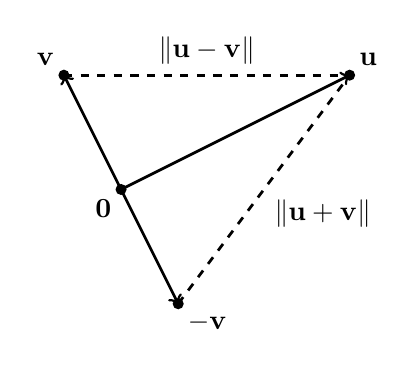
\begin{tikzpicture}[scale=1]
		% Set u and v
		\pgfmathsetmacro{\ux}{4}
		\pgfmathsetmacro{\uy}{2}
		\pgfmathsetmacro{\vx}{-1}
		\pgfmathsetmacro{\vy}{2}
		% Begin Axis
		\begin{axis}[axis lines=none,
		axis x line=center, axis y line=middle, 
		xmin=-2.5, xmax=5.5,
		ymin=-3.5, ymax=3.5,
		scale only axis, axis equal, height=2in,
		grid=major, grid style={line width=.5pt, draw=gray!50, dashed}]
		% Plot vectors
		\fill[black] (0,0) circle (2pt) node[below left, fill=white, rounded corners=0.2cm] {$\vect{0}$};
		\fill[black] (\ux,\uy) circle (2pt) node[above right, fill=white, rounded corners=0.2cm] {$\vect{u}$};
		\fill[black] (\vx,\vy) circle (2pt) node[above left, fill=white, rounded corners=0.2cm] {$\vect{v}$};
		\fill[black] (-\vx,-\vy) circle (2pt) node[below right, fill=white, rounded corners=0.2cm] {$-\vect{v}$};
		\draw[<->,line width=1pt] (\vx,\vy) -- (-\vx,-\vy);
		\draw[->,line width=1pt] (0,0) -- (\ux,\uy);
		\draw[dashed,line width=1pt] (\vx,\vy) -- (\ux,\uy) node[midway, above] {$\|\vect{u}-\vect{v}\|$};
		\draw[dashed,line width=1pt] (-\vx,-\vy) -- (\ux,\uy) node[midway, below right] {$\|\vect{u}+\vect{v}\|$};
		\end{axis}
		\end{tikzpicture}
		\vspace{3em}
		
		\item Determine if $\vect{u}$ and $\vect{v}$ are orthogonal by computing $\vect{u}\cdot\vect{v}$.
		\vspace{5em}
	\end{enumerate}
\end{exercise}


\begin{boxdef}
	If $\vect{z}$ is orthogonal to every vector in a subspace $W$, then we say $\vect{z}$ is \textbf{orthogonal} to $W$. The set of all $\vect{z}$ orthogonal to $W$ is called the \textbf{orthogonal complement} of $W$, denoted $W^\perp$. A vector $\vect{z}$ is in $W^\perp$ if, and only if, $\vect{z}$ is orthogonal to every vector in a spanning set for $W$.
\end{boxdef}

\begin{exercise} % 6.1.Custom
	Suppose $W$ is spanned by the set $\left\{ \begin{bmatrix}-4\\1\\-2\\6\end{bmatrix},\begin{bmatrix}2\\-5\\-1\\4\end{bmatrix} \right\}$. Is $\vect{u}=\begin{bmatrix}3\\2\\-5\\0\end{bmatrix}$ in $W^\perp$?
\end{exercise}
\vfill


\newpage


% SEC 6.2
\section{Orthogonal Sets}
\name

\begin{boxme}
	A set of vectors $\vectsetvp$ in $\R^n$ is said to be an \textbf{orthogonal set} if each pair of distinct vectors from the set is orthogonal, that is, if $\vect{v}_i\cdot\vect{v}_j=0$ whenever $i\neq j$.
\end{boxme}


\begin{exercise} % 6.2.4 (scaled)
	Determine if the set $\{\vect{u}_1,\vect{u}_2,\vect{u}_3\}$ is orthogonal.
	$$ \vect{u}_1 = \begin{bmatrix}2\\-2\\1\\2\end{bmatrix}, \quad
	\vect{u}_2 = \begin{bmatrix}-1\\4\\-4\\7\end{bmatrix}, \quad
	\vect{u}_3 = \begin{bmatrix}4\\7\\6\\0\end{bmatrix} $$
\end{exercise}
\vfill


\begin{boxthm}
	\textbf{Theorem 6.4.} \\
	If $S=\vectset[u]{1}{p}$ is an orthogonal set of nonzero vectors in $\R^n$, then $S$ is linearly independent and hence is a basis for the subspace spanned by $S$.
\end{boxthm}
\vspace{-1em}
\begin{boxthm}
	\textbf{Theorem 6.5.} \\
	Let $\vectset[u]{1}{p}$ be an orthogonal basis for a subspace $W$ of $\R^n$. For each $\vect{y}$ in $W$, the weights in the linear combination
	\vspace{-1ex}
	$$ \vect{y} = c_1\vect{u}_1+\cdots+c_p\vect{u}_p $$
	are given by 
	\vspace{-1ex}
	$$ c_j = \frac{\vect{y}\cdot\vect{u}_j}{\vect{u}_j\cdot\vect{u}_j} \qquad
	(\text{for } j=1,\ldots,p). $$
\end{boxthm}


\begin{exercise} % 6.2.10 (Don't have to check orthogonality)
	The set $\{\vect{u}_1,\vect{u}_2,\vect{u}_3\}$ is orthogonal. By Theorem 6.4 (and Theorem 2.15 or 4.12, The Basis Theorem), the set is a basis for $\R^3$. Write $\vect{x}$ as a linear combination of the basis vectors: $\vect{x} = c_1\vect{u}_1 + c_2\vect{u}_2 + c_3\vect{u}_3$.
	$$ \vect{u}_1 = \begin{bmatrix}2\\-2\\0\end{bmatrix}, \quad
	\vect{u}_2 = \begin{bmatrix}3\\3\\-1\end{bmatrix}, \quad
	\vect{u}_3 = \begin{bmatrix}1\\1\\6\end{bmatrix}, \quad
	\vect{x} = \begin{bmatrix}4\\-3\\1\end{bmatrix} $$
\end{exercise}
\vfill


\newpage


\begin{boxdef}
	Suppose $\vect{u}$ and $\vect{y}$ are given. It will be useful to write $\vect{y}=\yhat+\vect{z}$ where $\yhat$ is some scalar multiple of $\vect{u}$ and $\vect{z}$ is orthogonal to $\vect{u}$. The vector $\yhat$ is called the \textbf{orthogonal projection of $\vect{y}$ onto $\vect{u}$}, and the vector $\vect{z}$ is called the \textbf{component of $\vect{y}$ orthogonal to $\vect{u}$}.
	\vspace{-1em}
	\begin{multicols}{2}
		\begin{center}
		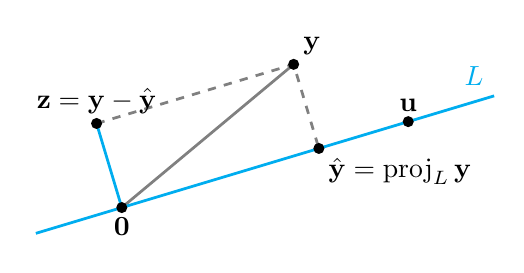
\begin{tikzpicture}[scale=1]
		% Set u and v
		\pgfmathsetmacro{\ux}{5}
		\pgfmathsetmacro{\uy}{1.5}
		\pgfmathsetmacro{\yx}{3}
		\pgfmathsetmacro{\yy}{2.5}
		\pgfmathparse{\yx*\ux+\yy*\uy}
		\pgfmathsetmacro{\ydotu}{\pgfmathresult}
		\pgfmathparse{\ux*\ux+\uy*\uy}
		\pgfmathsetmacro{\udotu}{\pgfmathresult}
		\pgfmathparse{\ydotu/\udotu*\ux}
		\pgfmathsetmacro{\yhatx}{\pgfmathresult}
		\pgfmathparse{\ydotu/\udotu*\uy}
		\pgfmathsetmacro{\yhaty}{\pgfmathresult}
		\pgfmathparse{\yx-\yhatx}
		\pgfmathsetmacro{\zx}{\pgfmathresult}
		\pgfmathparse{\yy-\yhaty}
		\pgfmathsetmacro{\zy}{\pgfmathresult}
		% Begin Axis
		\begin{axis}[axis lines=none,
		axis x line=center, axis y line=middle,
		xmin=-.5, xmax=5.5,
		ymin=-3.5, ymax=6.5,
		%	xtick={-3,...,5}, ytick={-3,...,7},
		%	xticklabels={,,}, yticklabels={,,},
		scale only axis, axis equal, % height=2in,
		gray, grid=major, grid style={line width=.5pt, draw=gray!50, dashed}]
		% Set Coordinates
		\coordinate (O) at (0,0);
		\coordinate (U) at (\ux,\uy);
		\coordinate (Y) at (\yx,\yy);
		\coordinate (YHAT) at (\yhatx,\yhaty);
		\coordinate (Z) at (\zx,\zy);
		% Connect Vectors
		\draw[line width=1pt] (O) -- (Y);
		\draw[cyan, line width=1pt] (O) -- (Z);
		\draw[dashed, line width=1pt] (Z) -- (Y) -- (YHAT);
		% Plot u and Span{u}
		\addplot[-, cyan, line width=1pt, domain=-1.5:6.5]{(\uy/\ux)*x} node[above left] {$L$};
		% Plot vectors
		\fill[black] (O) circle (2pt) node[below] {$\vect{0}$};
		\fill[black] (U) circle (2pt) node[above] {$\vect{u}$};
		\fill[black] (Y) circle (2pt) node[above right] {$\vect{y}$};
		\fill[black] (YHAT) circle (2pt) node[below right] {$\yhat=\proj_L\vect{y}$};
		\fill[black] (Z) circle (2pt) node[above] {$\vect{z}=\vect{y}-\yhat$};
		% ADD RIGHT ANGLE
		\end{axis}
		\end{tikzpicture}
		\end{center}

		\columnbreak
		
		If we let $L=\Span\{\vect{u}\}$, then we write
		$$ \yhat = \proj_L\vect{y} = \frac{\vect{y}\cdot\vect{u}}{\vect{u}\cdot\vect{u}}\vect{u} $$
	\end{multicols}
\end{boxdef}


\begin{exercise} % 6.2.12
	\begin{enumerate}[(a)]
		\item Compute the orthogonal projection of $\vect{y}=\begin{bmatrix}-4\\3\end{bmatrix}$ onto the line through $\vect{u}=\begin{bmatrix}-1\\4\end{bmatrix}$ and the origin.
		\vfill
		
		\item Using part (a), how could you compute the shortest distance from $\vect{y}$ to $L=\Span{\vect{u}}$?
		\vspace{3em}
	\end{enumerate}
\end{exercise}


\begin{boxdef}
	A set $\vectsetvp$ is an \textbf{orthonormal} if it is an orthogonal set of unit vectors. If $W=\Span\vectsetvp$, then the set is an \textbf{orthonormal basis} for $W$.
\end{boxdef}

\begin{exercise} % 6.2.17
	Determine if the set of vectors is orthonormal. If the set is only orthogonal, normalize the vectors to produce an orthonormal set.
	$$ \vect{u}_1 = \begin{bmatrix}2/3\\1/3\\1/3\end{bmatrix}, \quad
	\vect{u}_2 = \begin{bmatrix}1/\sqrt{5}\\0\\-2/\sqrt{5}\end{bmatrix} $$
\end{exercise}
\vfill


\newpage


% SEC 6.3
\section{Orthogonal Projections}
\name

\begin{boxthm}
	\textbf{Theorem 6.8.}
	\textbf{The Orthogonal Decomposition Theorem} \\
	Let $W$ be a subspace of $\R^n$. Then each $\vect{y}$ in $\R^n$ can be written uniquely in the form
	$ \vect{y} = \yhat+\vect{z} $
	where $\yhat$ is in $W$ and $\vect{z}$ is in $W^\perp$. In fact, if $\vectset[u]{1}{p}$ is any orthogonal basis of $W$, then
	$$ \yhat = \frac{\vect{y}\cdot\vect{u}_1}{\vect{u}_1\cdot\vect{u}_1}\vect{u}_1 + \cdots + \frac{\vect{y}\cdot\vect{u}_p}{\vect{u}_p\cdot\vect{u}_p}\vect{u}_p \qquad \text{and} \qquad \vect{z}=\vect{y}-\yhat. $$
	The vector $\yhat$ is called the \textbf{orthogonal projection of $\boldsymbol{\vect{y}}$ onto $\boldsymbol{W}$}, and the vector $\vect{z}$ is called the \textbf{component of $\boldsymbol{\vect{y}}$ orthogonal to $\boldsymbol{W}$}.
\end{boxthm}


\begin{exercise} % 6.3.5
	Verify that $\{\vect{u}_1,\vect{u}_2\}$ is an orthogonal set, and then find $\yhat$, the orthogonal projection of $\vect{y}$ onto $\Span\{\vect{u}_1,\vect{u}_2\}$. Hint: If you do the problem correctly, $\yhat$ has all integer entries.
	$$ \vect{y} = \begin{bmatrix}-1\\3\\6\end{bmatrix}, \quad
	\vect{u}_1 = \begin{bmatrix}-5\\-1\\-2\end{bmatrix}, \quad
	\vect{u}_2 = \begin{bmatrix}1\\-1\\-2\end{bmatrix}$$
\end{exercise}
\vfill


\begin{exercise} % 6.3.1
	Write $\vect{x}$ as the sum of two vectors, one in $\Span\{\vect{u}_1,\vect{u}_2,\vect{u}_3\}$ and the other in $\Span\{\vect{u}_4\}$. You may assume $\{\vect{u}_1,\vect{u}_2,\vect{u}_3,\vect{u}_4\}$ is an orthogonal basis for $\R^4$.
	$$ \vect{u}_1 = \begin{bmatrix}0\\1\\-4\\-1\end{bmatrix}, \quad
	\vect{u}_2 = \begin{bmatrix}3\\5\\1\\1\end{bmatrix}, \quad
	\vect{u}_3 = \begin{bmatrix}1\\0\\1\\-4\end{bmatrix}, \quad
	\vect{u}_4 = \begin{bmatrix}5\\-3\\-1\\1\end{bmatrix}, \quad
	\vect{x} = \begin{bmatrix}10\\-8\\2\\0\end{bmatrix}$$
	Hint: You could compute the orthogonal projections of $\vect{x}$ onto $\Span\{\vect{u}_1,\vect{u}_2,\vect{u}_3\}$ and $\Span\{\vect{u}_4\}$, but there is a much quicker method using Theorem 6.8. If we let $\xhat$ be the orthogonal projection of $\vect{x}$ onto $W=\Span\{\vect{u}_4\}$. Then $\vect{z}=\vect{x}-\xhat$ is in $W^\perp=\Span\{\vect{u}_1,\vect{u}_2,\vect{u}_3\}$. So $\vect{x}=\xhat+\vect{z}$ will be the sum you want.
\end{exercise}
\vfill


\newpage


\begin{boxthm}
	\textbf{Theorem 6.9.}
	\textbf{The Best Approximation Theorem} \\
	Let $W$ be a subspace of $\R^n$, let $\vect{y}$ be any vector in $\R^n$, and let $\yhat$ be the orthogonal projection of $\vect{y}$ onto $W$. Then $\yhat$ is the closest point in $W$ to $\vect{y}$, in the sense that
	$$ \|\vect{y}-\yhat\| < \|\vect{y}-\vect{v}\| $$
	for all $\vect{v}$ in $W$ distinct from $\yhat$. The vector $\yhat$ is \textbf{the best approximation to $\boldsymbol{\vect{y}}$ by elements of $\boldsymbol{W}$}.
\end{boxthm}


\begin{exercise} % 6.3.12
	Find the closest point to $\vect{y}$ in the subspace $W$ spanned by $\vect{v}_1$ and $\vect{v}_2$. Assume $\vect{v}_1$ and $\vect{v}_2$ are orthogonal.
	$$ \vect{y} = \begin{bmatrix}3\\-1\\1\\13\end{bmatrix}, \quad
	\vect{v}_1 = \begin{bmatrix}1\\-2\\-1\\2\end{bmatrix}, \quad
	\vect{v}_2 = \begin{bmatrix}-4\\1\\0\\3\end{bmatrix} $$
\end{exercise}
\vfill


\begin{boxthm}
	\textbf{Theorem 6.10.} \\
	If $\vectset[u]{1}{p}$ is an orthonormal basis for a subspace $W$ of $\R^n$, then
	$$ \proj_W\vect{y} = (\vect{y}\cdot\vect{u}_1)\vect{u}_1 + (\vect{y}\cdot\vect{u}_2)\vect{u}_2 + \cdots + (\vect{y}\cdot\vect{u}_p)\vect{u}_p. $$
	If $U=\begin{bmatrix}\vect{u}_1&\vect{u}_2&\cdots&\vect{u}_p\end{bmatrix}$, then
	$ \proj_W\vect{y} = UU^T\vect{y}$ for all $\vect{y}$ in $\R^n$.
\end{boxthm}


\begin{exercise} % 6.3.17
	Let $\vect{y}=\begin{bmatrix}4\\8\\1\end{bmatrix}$, $\vect{u}_1=\begin{bmatrix}2/3\\1/3\\2/3\end{bmatrix}$, $\vect{u}_2=\begin{bmatrix}-2/3\\2/3\\1/3\end{bmatrix}$, and $W=\Span\{\vect{u}_1,\vect{u}_2\}$. You may assume $\{\vect{u}_1,\vect{u}_2\}$ is orthonormal.
	\begin{enumerate}[(a)]
		\item Let $U=\begin{bmatrix}\vect{u}_1&\vect{u}_2\end{bmatrix}$ and compute $UU^T$.
		
		$UU^T = \begin{bmatrix}2/3&-2/3\\1/3&2/3\\2/3&1/3\end{bmatrix}
		\begin{bmatrix}2/3&1/3&2/3\\-2/3&2/3&1/3\end{bmatrix}=$
		\vspace{2em}
		\item Compute $\proj_W\vect{y}=UU^T\vect{y}$.
		\vspace{1in}
	\end{enumerate}
\end{exercise}


\newpage


% SEC 6.4
\section{The Gram-Schmidt Process}
\name

\begin{boxthm}
	\textbf{Theorem 6.11.}
	\textbf{The Gram-Schmidt Process} \\
	Given a basis $\vectset[x]{1}{p}$ for a nonzero subspace $W$ of $\R^n$, define
	\vspace{-1ex}
	\begin{align*}
	\vect{v}_1 &= \vect{x}_1 \\
	\vect{v}_2 &= \vect{x}_2 - \frac{\vect{x}_2\cdot\vect{v}_1}{\vect{v}_1\cdot\vect{v}_1}\vect{v}_1 \\
	\vect{v}_3 &= \vect{x}_3 - \frac{\vect{x}_3\cdot\vect{v}_1}{\vect{v}_1\cdot\vect{v}_1}\vect{v}_1 - \frac{\vect{x}_3\cdot\vect{v}_2}{\vect{v}_2\cdot\vect{v}_2}\vect{v}_2 \\
	&\vdots \\
	\vect{v}_p &= \vect{x}_p - \frac{\vect{x}_p\cdot\vect{v}_1}{\vect{v}_1\cdot\vect{v}_1}\vect{v}_1 - \frac{\vect{x}_p\cdot\vect{v}_2}{\vect{v}_2\cdot\vect{v}_2}\vect{v}_2 - \ldots -  \frac{\vect{x}_p\cdot\vect{v}_{p-1}}{\vect{v}_{p-1}\cdot\vect{v}_{p-1}}\vect{v}_{p-1}.
	\end{align*}
	Then $\vectsetvp$ is an orthogonal basis for $W$, and $\Span\vectset{1}{k} = \Span\vectset[x]{1}{k}$ for $k\leq p$.
\end{boxthm}


\begin{exercise} % 6.4.3
	The set $\{\vect{x}_1,\vect{x}_2\}$ is a basis for a subspace $W$. Use the Gram-Schmidt process to produce an orthogonal basis for $W$. Hint: Scaling vectors before you begin may simplify calculations.
	
	\vspace{1em}
	$ \vect{x}_1 = \begin{bmatrix}2\\-5\\4\end{bmatrix}, \quad
	\vect{x}_2 = \begin{bmatrix}6\\-6\\3\end{bmatrix} $
\end{exercise}
\vfill


\begin{exercise} % 6.4.10 (altered)
	A matrix $A$ with linearly independent columns is given below. Find an orthogonal basis for the column space of $A$. Note that columns 1 and 2 are already orthogonal. Hint: Recall that one possible basis for $\Col A$ consists of the pivot columns of $A$.
	
	\vspace{1em}
	$ A = \begin{bmatrix}-1&1&3\\3&0&1\\2&1&3\\1&-1&-1\end{bmatrix} $
\end{exercise}
\vfill


\newpage


\begin{exercise} % 6.4.8
	The set $\{\vect{v}_1,\vect{v}_2\}$ is an orthogonal basis for a subspace $W$. Find an orthonormal basis for $W$. Hint: Since scaling vectors does not affect orthogonality, you may wish to scale $\vect{v}_1$ and $\vect{v}_2$ before normalizing.
	
	\vspace{1em}
	$ \vect{v}_1 = \begin{bmatrix}2\\-6\\4\end{bmatrix}, \quad
	\vect{v}_2 = \begin{bmatrix}-5\\-5\\-5\end{bmatrix} $
\end{exercise}
\vspace{1.75in}


\begin{boxthm}
	\textbf{Theorem 6.12.}
	\textbf{The $\boldsymbol{QR}$ Factorization} \\
	If $A$ is an $m\times n$ matrix with linearly independent columns, then $A$ can be factored as $A=QR$, where $Q$ is an $m\times n$ matrix whose columns form an orthonormal basis for $\Col A$ and $R$ is an $n\times n$ upper triangular invertible matrix with positive entries on its diagonal.
\end{boxthm}
\vspace{-1em}
\begin{boxme}
	To produce $Q$, orthogonalize and normalize the columns of $A$, i.e., apply the Gram-Schmidt process (with normalization) to the columns of $A$. To produce $R$, use the following:
	\vspace{-1em}
	\begin{align*}
	QR &= A \\
	Q^TQR &= Q^TA \\
	IR &= Q^TA &\text{(By Thm 6.6, since $Q$ has orthonormal columns, $Q^TQ=I$)}\\
	R &= Q^TA
	\end{align*}
\end{boxme}


\begin{exercise} % 6.4.14
	The columns of $Q$ were obtained by applying the Gram-Schmidt process (with normalization) to the columns of $A$. Find an upper triangular matrix $R$ such that $A=QR$.
	
	\vspace{1em}
	$ A= \begin{bmatrix}-2&-3\\5&7\\-2&-2\\-4&-1\end{bmatrix}, \quad
	Q= \begin{bmatrix}-2/7&-1/\sqrt{14}\\5/7&2/\sqrt{14}\\-2/7&0\\-4/7&3/\sqrt{14}\\\end{bmatrix}$
%	\begin{align*}
%	A &= \begin{bmatrix}-2&-3\\5&7\\-2&-2\\-4&-1\end{bmatrix} &
%	Q &= \begin{bmatrix}-2/7&-1/\sqrt{14}\\5/7&2/\sqrt{14}\\-2/7&0\\-4/7&3/\sqrt{14}\\\end{bmatrix}
%	\end{align*}
\end{exercise}
\vfill


\newpage


% SEC 6.5
\section{Least-Squares Problems}
\name

%\begin{boxdef}
%If $A$ is $m\times n$ and $\vect{b}$ is in $\R^m$, a \textbf{least-squares solution} of $\Axb$ is an $\xhat$ in $\R^n$ such that
%\vspace{-1ex}
%$$ \|\vect{b}-A\xhat\| \leq \|\vect{b}-A\vect{x}\| \qquad
%\text{for all $\vect{x}$ in $\R^n$.} $$
%\end{boxdef}

\begin{boxthm}
	\textbf{Theorem 6.13.} \\
	The set of least-squares solutions of $\Axb$ coincides with the nonempty set of solutions of the normal equations $\NormEq$.
\end{boxthm}


\begin{exercise} % 6.5.5
	Describe all the least-squares solutions of the equation $\Axb$.
	\begin{multicols}{2}
		$ A = \begin{bmatrix}1&1&0\\1&1&0\\1&0&1\\1&0&1\end{bmatrix}, 
		\vect{b} = \begin{bmatrix}2\\6\\5\\1\end{bmatrix} $
		\begin{enumerate}[(a)]
			\item Compute $A^TA$ and $A^T\vect{b}$. \\
			$ A^TA = \begin{bmatrix}1&1&1&1\\1&1&0&0\\0&0&1&1\end{bmatrix} \begin{bmatrix}1&1&0\\1&1&0\\1&0&1\\1&0&1\end{bmatrix} = $
			
			\vspace{2em}
			$ A^T\vect{b} = \begin{bmatrix}1&1&1&1\\1&1&0&0\\0&0&1&1\end{bmatrix} \begin{bmatrix}2\\6\\5\\1\end{bmatrix} = $
			\columnbreak
			\item Solve $\NormEq$. \\
			(You may use a calculator or computer)
		\end{enumerate}
	\end{multicols}
\end{exercise}
\vspace{2em}


\begin{boxthm}
	\textbf{Theorem 6.14.} \\
	Let $A$ be an $m\times n$ matrix. The following statements are logically equivalent:
	\vspace{-1ex}
	\begin{enumerate}[(a)]\itemsep=0em
		\item The equation $\Axb$ has a unique least-squares solution for each $\vect{b}$ in $\R^m$.
		\item The columns of $A$ are linearly independent.
		\item The matrix $A^TA$ is invertible.
	\end{enumerate}
	\vspace{-1ex}
	When these statements are true, the least-squares solution $\xhat$ is given by
	$ \xhat = \left(A^TA\right)^{-1}A^T\vect{b}. $
\end{boxthm}


\begin{exercise} % 6.5.1
	Find a least-squares solution of $\Axb$. Use Theorem 6.14 if applicable. \par
	$ A = \begin{bmatrix}-1&2\\2&-3\\-1&3\end{bmatrix}, 
	\vect{b} = \begin{bmatrix}16\\4\\8\end{bmatrix} $
	
	\begin{multicols}{2}
	\begin{align*}
	A^TA &= \begin{bmatrix}-1&2&-1\\2&-3&3\end{bmatrix}
	\begin{bmatrix}-1&2\\2&-3\\-1 &3\end{bmatrix} \\
	&= \begin{bmatrix}6&-11\\-11&22\end{bmatrix} \\[1em]
	A^T\vect{b} &= \begin{bmatrix}-1&2&-1\\2&-3&3\end{bmatrix} \begin{bmatrix}16\\4\\8\end{bmatrix} = \begin{bmatrix}-16\\44\end{bmatrix}
	\end{align*}
	
	\columnbreak
	\end{multicols}
\end{exercise}
\vfill


\newpage


\begin{exercise} % 6.5.10
	Let $ A = \begin{bmatrix}1&2\\-1&4\\1&2\end{bmatrix} $ and $ \vect{b} = \begin{bmatrix}2\\-1\\6\end{bmatrix} $.
	\begin{enumerate}[(a)]
		\item Find the orthogonal projection of $\vect{b}$ onto $\Col A$. Note that the columns of $A$ are linearly independent and orthogonal, so you already have an orthogonal basis for $\Col A$.
		\vspace{1.75in}
		\item Use your calculations in part (a) to find a least-squares solution of $\Axb$. \par Hint: Think of the entries of $\vect{x}$ as weights for a linear combination of the columns of $A$.
		\vspace{4em}
	\end{enumerate}
\end{exercise}


\begin{boxthm}
	\textbf{Theorem 6.15.} \\
	Given an $m\times n$ matrix $A$ with linearly independent columns, let $A=QR$ be a $QR$ factorization of $A$ as in Theorem 6.12. Then, for each $\vect{b}$ in $\R^m$, the equation $\Axb$ has a unique least-squares solution, given by
	\vspace{-1em}
	\begin{align*}
	\xhat &= R^{-1}Q^T\vect{b}. &
	(\text{Numerical Note: it is usually much quicker to solve } R\xhat = Q^T\vect{b}.)
	\end{align*}
\end{boxthm}


\begin{exercise} % 6.5.15
	Use the factorization $A=QR$ given below to find the least-squares solution of $\Axb$.
	\begin{align*}
	A &= \begin{bmatrix}2&3\\2&4\\1&1\end{bmatrix} =
	\begin{bmatrix}2/3&-1/3\\2/3&2/3\\1/3&-2/3\end{bmatrix}
	\begin{bmatrix}3&5\\0&1\end{bmatrix} &
	\vect{b} &= \begin{bmatrix}6\\3\\9\end{bmatrix}
	\end{align*}
	\begin{enumerate}[(a)]
		\item Compute $Q^T\vect{b}$. \par
		$ Q^T\vect{b}= \begin{bmatrix}2/3&2/3&1/3\\-1/3&2/3&-2/3\end{bmatrix}
		\begin{bmatrix}6\\3\\9\end{bmatrix} = $
		\vspace{2em}
		\item Solve $R\xhat=Q^T\vect{b}$ via back-substitution.
		\vspace{1in}
	\end{enumerate}
\end{exercise}


\newpage


% CH 7
\chapter{Symmetric Matrices and Quadratic Forms}
\chaptermark{Symmetric Matrices \& Quad. Forms}

% SEC 7.1
\section[Diag. of Sym. Matrices]{Diagonalization of Symmetric Matrices}
\name[1.5in]

\begin{boxdef}
	A \textbf{symmetric matrix} is a matrix $A$ such that $A^T=A$.
\end{boxdef}
\vspace{-1em}
\begin{boxthm}
	\textbf{Theorem 7.1.} \\
	If $A$ is symmetric, then any two eigenvectors from different eigenspaces are orthogonal.
\end{boxthm}


\begin{exercise} % 7.1.19 Custom
	\begin{enumerate}[(a)]
		\item Fill in the following matrix so that it is symmetric:
%		$$ A = \begin{bmatrix}2&-4&8\\-4&8&4\\8&4&2\end{bmatrix} $$	
		\begingroup
		\renewcommand{\arraystretch}{1.5}
		$$ A = \begin{bmatrix}2&&  &&8\\-4&&8&&4\\ && &&2\end{bmatrix} $$
		\endgroup
		\item The vectors $\vect{v}_1=\begin{bmatrix}-1\\2\\0\end{bmatrix}$, $\vect{v}_2=\begin{bmatrix}1\\0\\1\end{bmatrix}$, and $\vect{v}_3=\begin{bmatrix}2\\1\\-2\end{bmatrix}$ are eigenvectors of the symmetric matrix $A$ above. The eigenvalue for $\vect{v}_1$ and $\vect{v}_2$ is $\lambda=10$, and the eigenvalue for $\vect{v}_3$ is $\lambda=-8$. What does Theorem 7.1 tell you about $\vect{v}_1\cdot\vect{v}_2$, $\vect{v}_2\cdot\vect{v}_3$, and $\vect{v}_1\cdot\vect{v}_3$, if anything?
	\end{enumerate}
\end{exercise}
\vspace{2in}


\begin{boxdef}
	An \textbf{orthogonal matrix} (section 6.2) is a square matrix $A$ with orthonormal columns (so $A^{-1}=A^T$). \par
	A matrix $A$ is \textbf{orthogonally diagonalizable} if there are an orthogonal matrix $P$ and a diagonal matrix $D$ such that $A=PDP^{-1}=PDP^T$.
\end{boxdef}
\vspace{-1em}
\begin{boxthm}
	\textbf{Theorem 7.2.} \\
	An $n\times n$ matrix $A$ is orthogonally diagonalizable if, and only if, $A$ is a symmetric matrix.
\end{boxthm}


\begin{exercise} % 7.1.9 Custom
	\begin{enumerate}[(a)]
		\item Is $B$ an orthogonal matrix? Why or why not? \par
		$ B = \begin{bmatrix}2&-3\\3&2\end{bmatrix} $
		\item Give an example of a $3\times 3$ matrix that is orthogonally diagonalizable.
	\end{enumerate}
\end{exercise}
\vfill


\newpage


\begin{boxme}
	\textbf{Steps to Orthogonally Diagonalize an $\boldsymbol{n\times n}$ Symmetric Matrix}
	\begin{enumerate}[(i)]\itemsep=0em
		\item Find the eigenvalues of $A$ 
		\item Find $n$ linearly independent eigenvectors for $A$, orthogonalize the set (if necessary), and normalize
		\item Construct $P$ from the orthonormalized eigenvectors you obtain in step (ii)
		\item Construct $D$ by placing the corresponding eigenvectors along the diagonal of $D$
	\end{enumerate}
\end{boxme}


\begin{exercise} % 7.1.15 Custom
	A matrix and two eigenvectors are given below. Orthogonally diagonalize the matrix (you only need to determine $P$ and $D$). Steps (i) and (ii) should go quickly since you already have 2 eigenvectors. \par
	$ A = \begin{bmatrix}13&4\\4&7\end{bmatrix}, 
	\vect{v}_1 = \begin{bmatrix}-1\\2\end{bmatrix}, 
	\vect{v}_2 = \begin{bmatrix}2\\1\end{bmatrix} $
%	\begin{align*}
%	A &= \begin{bmatrix}13&4\\4&7\end{bmatrix} &
%	\vect{v}_1 &= \begin{bmatrix}-1\\2\end{bmatrix}, 
%	\vect{v}_2 = \begin{bmatrix}2\\1\end{bmatrix}
%	\end{align*}
\end{exercise}
\vfill


\begin{boxdef}
	The set of eigenvalues of a matrix $A$ is called the \textbf{spectrum} of $A$. A \textbf{spectral decomposition} for $A$ can be obtained from the columns of $P$ and eigenvalues from $D$ in the orthogonal diagonalization of $A$:
	\begin{align*}
	A &= PDP^T
	= \begin{bmatrix}\vect{u}_1&\cdots&\vect{u}_n\end{bmatrix}
	\begin{bmatrix}\lambda_1&&0\\&\ddots&\\0&&\lambda_n\end{bmatrix}
	\begin{bmatrix}[c]\vect{u}_1^T\\ \vdots\\ \vect{u}_n^T\end{bmatrix}
	= \begin{bmatrix}\lambda_1\vect{u}_1&\cdots&\lambda_n\vect{u}_n\end{bmatrix}
	\begin{bmatrix}[c]\vect{u}_1^T\\ \vdots\\ \vect{u}_n^T\end{bmatrix}
	\end{align*}
	This last expression can be rewritten as a spectral decomposition:
	$A = \lambda_1\vect{u}_1\vect{u}_1^T + \lambda_2\vect{u}_2\vect{u}_2^T + \cdots + \lambda_n\vect{u}_n\vect{u}_n^T.$ This is a sum of matrices each of which relies on just one column of $P$ and its corresponding eigenvalue.
\end{boxdef}


\begin{exercise} % 7.1.15 Custom
	Find a spectral decomposition for the matrix $A$ using the given orthogonal diagonalization, $A=PDP^T$.
	\begin{align*}
	A &= \begin{bmatrix}2&9\\9&2\end{bmatrix} &
	PDP^T &= 
	\begin{bmatrix}-1/\sqrt{2}&1/\sqrt{2}\\1/\sqrt{2}&1/\sqrt{2}\end{bmatrix}
	\begin{bmatrix}-7&0\\0&11\end{bmatrix}
	\begin{bmatrix}-1/\sqrt{2}&1/\sqrt{2}\\1/\sqrt{2}&1/\sqrt{2}\end{bmatrix}
	\end{align*}
	\begin{enumerate}[(a)]
		\item Compute $\vect{u}_1\vect{u}_1^T$ and $\vect{u}_2\vect{u}_2^T$, where $\vect{u}_1$ and $\vect{u}_2$ are the first and second columns of $P$, respectively.
		\vspace{1in}
		\item Write a spectral decomposition for $A$.
		\vspace{3em}
	\end{enumerate}
\end{exercise}


%\newpage
%
%
%% SEC 7.2
%\section{Quadratic Forms}
%\name
%
%\begin{exercise} % 7.2.
%	Text here.
%\end{exercise}
%\vfill
%
%
%\begin{exercise} % 7.2.
%	Text here.
%\end{exercise}
%\vfill
%
%
%\newpage
%
%
%\begin{exercise} % 7.2.
%	Text here.
%\end{exercise}
%\vfill
%
%
%\begin{exercise} % 7.2.
%	Text here.
%\end{exercise}
%\vfill
%
%
%\newpage
%
%
%\setcounter{section}{3}
%\section{The Singular Value Decomposition}
%\name
%
%\begin{exercise} % 7.4.
%	Text here.
%\end{exercise}
%\vfill
%
%
%\begin{exercise} % 7.4.
%	Text here.
%\end{exercise}
%\vfill
%
%
%\newpage
%
%
%\begin{exercise} % 7.4.
%	Text here.
%\end{exercise}
%\vfill
%
%
%\begin{exercise} % 7.4.
%	Text here.
%\end{exercise}
%\vfill


\end{document}



% Exercise Template:
\begin{exercise} % 7.X.
	Text here.
\end{exercise}
\vfill

% System template
$\systeme{
	x_1				-	3x_3 =  8,
	2x_1	+	2x_2	+	9x_3 =  7,
	x_2	+	5x_3 = -2}$
